\PassOptionsToPackage{unicode=true}{hyperref} % options for packages loaded elsewhere
\PassOptionsToPackage{hyphens}{url}
%
\documentclass{article}

\usepackage{graphicx} % For including images
\usepackage{titlesec} % For formatting section titles

\usepackage{lmodern}
\renewcommand{\normalsize}{\fontsize{9}{10.8}\selectfont}

\usepackage{placeins}
\usepackage{epstopdf}
\usepackage{listings} % For code blocks
\usepackage{xcolor}   % For color customization
\usepackage{longtable}
\usepackage[a4paper, margin=1in]{geometry} % Adjust margins here
\usepackage{amssymb,amsmath}
\usepackage{ifxetex,ifluatex}
\usepackage{fixltx2e} % provides \textsubscript
\ifnum 0\ifxetex 1\fi\ifluatex 1\fi=0 % if pdftex
  \usepackage[T1]{fontenc}
  \usepackage[utf8]{inputenc}
  \usepackage{textcomp} % provides euro and other symbols
\else % if luatex or xelatex
  \usepackage{unicode-math}
  \defaultfontfeatures{Ligatures=TeX,Scale=MatchLowercase}
\fi
% use upquote if available, for straight quotes in verbatim environments
\IfFileExists{upquote.sty}{\usepackage{upquote}}{}
% use microtype if available
\IfFileExists{microtype.sty}{%
\usepackage[]{microtype}
\UseMicrotypeSet[protrusion]{basicmath} % disable protrusion for tt fonts
}{}
\IfFileExists{parskip.sty}{%
\usepackage{parskip}
}{% else
\setlength{\parindent}{0pt}
\setlength{\parskip}{6pt plus 2pt minus 1pt}
}
\usepackage[colorlinks=true, linkcolor=blue, urlcolor=blue, citecolor=blue]{hyperref}
\hypersetup{
            pdfborder={0 0 0},
            breaklinks=true}
\urlstyle{same}  % don't use monospace font for urls
\usepackage{color}
\usepackage{fancyvrb}
\newcommand{\VerbBar}{|}
\newcommand{\VERB}{\Verb[commandchars=\\\{\}]}
\DefineVerbatimEnvironment{Highlighting}{Verbatim}{commandchars=\\\{\}}
% Add ',fontsize=\small' for more characters per line
\usepackage{framed}
\definecolor{shadecolor}{RGB}{42,33,28}
\newenvironment{Shaded}{\begin{snugshade}}{\end{snugshade}}
\newcommand{\AlertTok}[1]{\textcolor[rgb]{1.00,1.00,0.00}{#1}}
\newcommand{\AnnotationTok}[1]{\textcolor[rgb]{0.00,0.40,1.00}{\textbf{\textit{#1}}}}
\newcommand{\AttributeTok}[1]{\textcolor[rgb]{0.74,0.68,0.62}{#1}}
\newcommand{\BaseNTok}[1]{\textcolor[rgb]{0.27,0.67,0.26}{#1}}
\newcommand{\BuiltInTok}[1]{\textcolor[rgb]{0.74,0.68,0.62}{#1}}
\newcommand{\CharTok}[1]{\textcolor[rgb]{0.02,0.61,0.04}{#1}}
\newcommand{\CommentTok}[1]{\textcolor[rgb]{0.00,0.40,1.00}{\textbf{\textit{#1}}}}
\newcommand{\CommentVarTok}[1]{\textcolor[rgb]{0.74,0.68,0.62}{#1}}
\newcommand{\ConstantTok}[1]{\textcolor[rgb]{0.74,0.68,0.62}{#1}}
\newcommand{\ControlFlowTok}[1]{\textcolor[rgb]{0.26,0.66,0.93}{\textbf{#1}}}
\newcommand{\DataTypeTok}[1]{\textcolor[rgb]{0.74,0.68,0.62}{\underline{#1}}}
\newcommand{\DecValTok}[1]{\textcolor[rgb]{0.27,0.67,0.26}{#1}}
\newcommand{\DocumentationTok}[1]{\textcolor[rgb]{0.00,0.40,1.00}{\textit{#1}}}
\newcommand{\ErrorTok}[1]{\textcolor[rgb]{1.00,1.00,0.00}{\textbf{#1}}}
\newcommand{\ExtensionTok}[1]{\textcolor[rgb]{0.74,0.68,0.62}{#1}}
\newcommand{\FloatTok}[1]{\textcolor[rgb]{0.27,0.67,0.26}{#1}}
\newcommand{\FunctionTok}[1]{\textcolor[rgb]{1.00,0.58,0.35}{\textbf{#1}}}
\newcommand{\ImportTok}[1]{\textcolor[rgb]{0.74,0.68,0.62}{#1}}
\newcommand{\InformationTok}[1]{\textcolor[rgb]{0.00,0.40,1.00}{\textbf{\textit{#1}}}}
\newcommand{\KeywordTok}[1]{\textcolor[rgb]{0.26,0.66,0.93}{\textbf{#1}}}
\newcommand{\NormalTok}[1]{\textcolor[rgb]{0.74,0.68,0.62}{#1}}
\newcommand{\OperatorTok}[1]{\textcolor[rgb]{0.74,0.68,0.62}{#1}}
\newcommand{\OtherTok}[1]{\textcolor[rgb]{0.74,0.68,0.62}{#1}}
\newcommand{\PreprocessorTok}[1]{\textcolor[rgb]{0.74,0.68,0.62}{\textbf{#1}}}
\newcommand{\RegionMarkerTok}[1]{\textcolor[rgb]{0.74,0.68,0.62}{#1}}
\newcommand{\SpecialCharTok}[1]{\textcolor[rgb]{0.02,0.61,0.04}{#1}}
\newcommand{\SpecialStringTok}[1]{\textcolor[rgb]{0.02,0.61,0.04}{#1}}
\newcommand{\StringTok}[1]{\textcolor[rgb]{0.02,0.61,0.04}{#1}}
\newcommand{\VariableTok}[1]{\textcolor[rgb]{0.74,0.68,0.62}{#1}}
\newcommand{\VerbatimStringTok}[1]{\textcolor[rgb]{0.02,0.61,0.04}{#1}}
\newcommand{\WarningTok}[1]{\textcolor[rgb]{1.00,1.00,0.00}{\textbf{#1}}}
\usepackage{longtable,booktabs}
% Fix footnotes in tables (requires footnote package)
\IfFileExists{footnote.sty}{\usepackage{footnote}\makesavenoteenv{longtable}}{}
\setlength{\emergencystretch}{3em}  % prevent overfull lines
\providecommand{\tightlist}{%
  \setlength{\itemsep}{0pt}\setlength{\parskip}{0pt}}
\setcounter{secnumdepth}{2}
% Redefines (sub)paragraphs to behave more like sections
\ifx\paragraph\undefined\else
\let\oldparagraph\paragraph
\renewcommand{\paragraph}[1]{\oldparagraph{#1}\mbox{}}
\fi
\ifx\subparagraph\undefined\else
\let\oldsubparagraph\subparagraph
\renewcommand{\subparagraph}[1]{\oldsubparagraph{#1}\mbox{}}
\fi


%\begin{scriptsize}
%\begin{Shaded}
%\begin{Highlighting}[]
%\NormalTok{$ }\BuiltInTok{\ExtensionTok{python\ test\_gsm.py\ -\/-load\ \textless{}gs\_checkpoint\_path\textgreater{}}}   
%\end{Highlighting}
%\end{Shaded}
%\end{scriptsize}

\newcommand{\codeline}[1]{\texttt{\NormalTok{\$ }\BuiltInTok{\ExtensionTok{#1}}}}
\newenvironment{codeblock}
{
\begin{scriptsize}
\begin{Shaded}
}
{
\end{Shaded}
\end{scriptsize}
}


% set default figure placement to htbp
\makeatletter
\def\fps@figure{htbp}
\makeatother


\title{pySLAM: An Open-Source, Modular, and Extensible Framework for SLAM}
\author{Luigi Freda}
\date{\small \today}  % put the 

\begin{document}

\maketitle
\begin{center}
  \href{https://github.com/luigifreda/pyslam}{github.com/luigifreda/pyslam}
\end{center}

\begin{abstract}
pySLAM is an open-source Python framework for Visual SLAM that supports monocular, stereo, and RGB-D camera inputs. It offers a flexible and modular interface, integrating a broad range of both classical and learning-based local features. The framework includes multiple loop closure strategies, a volumetric reconstruction pipeline, and support for depth prediction models. It also offers a comprehensive set of tools for the experimentation and evaluation of visual odometry and SLAM modules.
Designed for both beginners and experienced researchers, pySLAM emphasizes rapid prototyping, extensibility, and reproducibility across diverse datasets. Its modular architecture facilitates the integration of custom components and encourages research that bridges traditional and deep learning-based approaches. Community contributions are welcomed, fostering collaborative development and innovation in the field of Visual SLAM.
This document\footnote{You may find an updated version of this document at:\\ \href{https://github.com/luigifreda/pyslam/blob/master/docs/tex/document.pdf}{github.com/luigifreda/pyslam/blob/master/docs/tex/document.pdf}} presents the pySLAM framework, outlining its main components, features, and usage.
\end{abstract}

\begin{figure}[htbp]
  \centering
  \includegraphics[width=0.5\textwidth]{images_tex/pyslam-teaser-rect.png}
  \label{fig:teaser}
\end{figure}

\tableofcontents

\pagebreak

\section{Introduction}

The objective of this document is to present the pySLAM framework, its main features, and usage\footnote{You may find an updated version of this document at:\\ \href{https://github.com/luigifreda/pyslam/blob/master/docs/tex/document.pdf}{github.com/luigifreda/pyslam/blob/master/docs/tex/document.pdf}}. \textbf{pySLAM} is a python implementation of a \emph{Visual SLAM} pipeline that supports \textbf{monocular}, \textbf{stereo} and
\textbf{RGBD} cameras. It provides the following \textbf{features} in a single python environment: 

\begin{itemize}
    \item A wide range of classical and modern
    \textbf{\protect\hyperlink{supported-local-features}{local features}}
    with a convenient interface for their integration. 
    
    \item Various loop closing methods, including
    \textbf{\protect\hyperlink{supported-global-descriptors-and-local-descriptor-aggregation-methods}{descriptor
    aggregators}} such as visual Bag of Words (BoW, iBow), Vector of Locally
    Aggregated Descriptors (VLAD), and modern
    \textbf{\protect\hyperlink{supported-global-descriptors-and-local-descriptor-aggregation-methods}{global
    descriptors}} (image-wise descriptors).
    
    \item A
    \textbf{\protect\hyperlink{volumetric-reconstruction}{volumetric
    reconstruction pipeline}} that processes available depth and color
    images with volumetric integration and provides an output dense
    reconstruction. This can use \textbf{TSDF} with voxel hashing or
    incremental \textbf{Gaussian Splatting}.
    
    \item Integration of
    \textbf{\protect\hyperlink{depth-prediction}{depth prediction models}}
    within the SLAM pipeline. These include DepthPro, DepthAnythingV2,
    RAFT-Stereo, CREStereo, MASt3R, MVDUSt3R, etc.

    \item A suite of segmentation models for
    \textbf{\protect\hyperlink{semantic-mapping}{semantic understanding}} of
    the scene, such as DeepLabv3, Segformer, and dense CLIP.
    
    \item Additional tools for VO (Visual Odometry) and SLAM, with built-in
    support for both \textbf{g2o} and \textbf{GTSAM}, along with custom
    Python bindings for features not included in the original libraries

    \item Built-in support for over \textbf{\protect\hyperlink{datasets}{10 dataset
    types}}.
\end{itemize}

pySLAM serves as flexible baseline framework to experiment with VO/SLAM
techniques, \emph{\protect\hyperlink{supported-local-features}{local
features}},
\emph{\protect\hyperlink{supported-global-descriptors-and-local-descriptor-aggregation-methods}{descriptor
aggregators}},
\emph{\protect\hyperlink{supported-global-descriptors-and-local-descriptor-aggregation-methods}{global
descriptors}},
\emph{\protect\hyperlink{volumetric-reconstruction-pipeline}{volumetric
integration}}, \emph{\protect\hyperlink{depth-prediction}{depth
prediction}} and \emph{\protect\hyperlink{semantic-mapping}{semantic
mapping}}. It allows to explore, prototype and develop VO/SLAM
pipelines. pySLAM is a research framework and a work in progress. It is
not optimized for real-time performances.

\textbf{Enjoy it!}


\hypertarget{system_overview}{%
\section{Overview}}

\subsection{Main Scritps}

A convenient entry-point are the following \textbf{main scripts}:
\begin{itemize}
\item 
\texttt{main\_vo.py} combines the simplest VO
ingredients without performing any image point triangulation or windowed
bundle adjustment. At each step \(k\), \texttt{main\_vo.py} estimates
the current camera pose \(C_k\) with respect to the previous one
\(C_{k-1}\). The inter-frame pose estimation returns
\([R_{k-1,k},t_{k-1,k}]\) with \(\Vert t_{k-1,k} \Vert=1\). With this
very basic approach, you need to use a ground truth in order to recover
a correct inter-frame scale \(s\) and estimate a valid trajectory by
composing \(C_k = C_{k-1} [R_{k-1,k}, s t_{k-1,k}]\). This script is a
first start to understand the basics of inter-frame feature tracking and
camera pose estimation.
\item
  \texttt{main\_slam.py} adds feature tracking along multiple frames,
  point triangulation, keyframe management, bundle adjustment, loop
  closing, dense mapping and depth inference in order to estimate the
  camera trajectory and build both a sparse and dense map. It's a full
  SLAM pipeline and includes all the basic and advanced blocks which are
  necessary to develop a real visual SLAM pipeline.
\item
  \texttt{main\_feature\_matching.py} shows how to use the basic feature
  tracker capabilities (\emph{feature detector} + \emph{feature
  descriptor} + \emph{feature matcher}) and allows to test the different
  available local features.
\item
  \texttt{main\_depth\_prediction.py} shows how to use the available
  depth inference models to get depth estimations from input color
  images.
\item
  \texttt{main\_map\_viewer.py} reloads a saved map and visualizes it.
  Further details on how to save a map
  \protect\hyperlink{reload-a-saved-map-and-relocalize-in-it}{here}.
\item
  \texttt{main\_map\_dense\_reconstruction.py} reloads a saved map and
  uses a configured volumetric integrator to obtain a dense
  reconstruction (see
  \protect\hyperlink{volumetric-reconstruction}{here}).
  \item
  \texttt{main\_slam\_evaluation.py} enables automated SLAM evaluation
  by executing \texttt{main\_slam.py} across a collection of datasets
  and configuration presets (see
  \protect\hyperlink{evaluating-slam}{here}).
\end{itemize}

\newpage

\begin{figure}[!t]
\begin{center}
    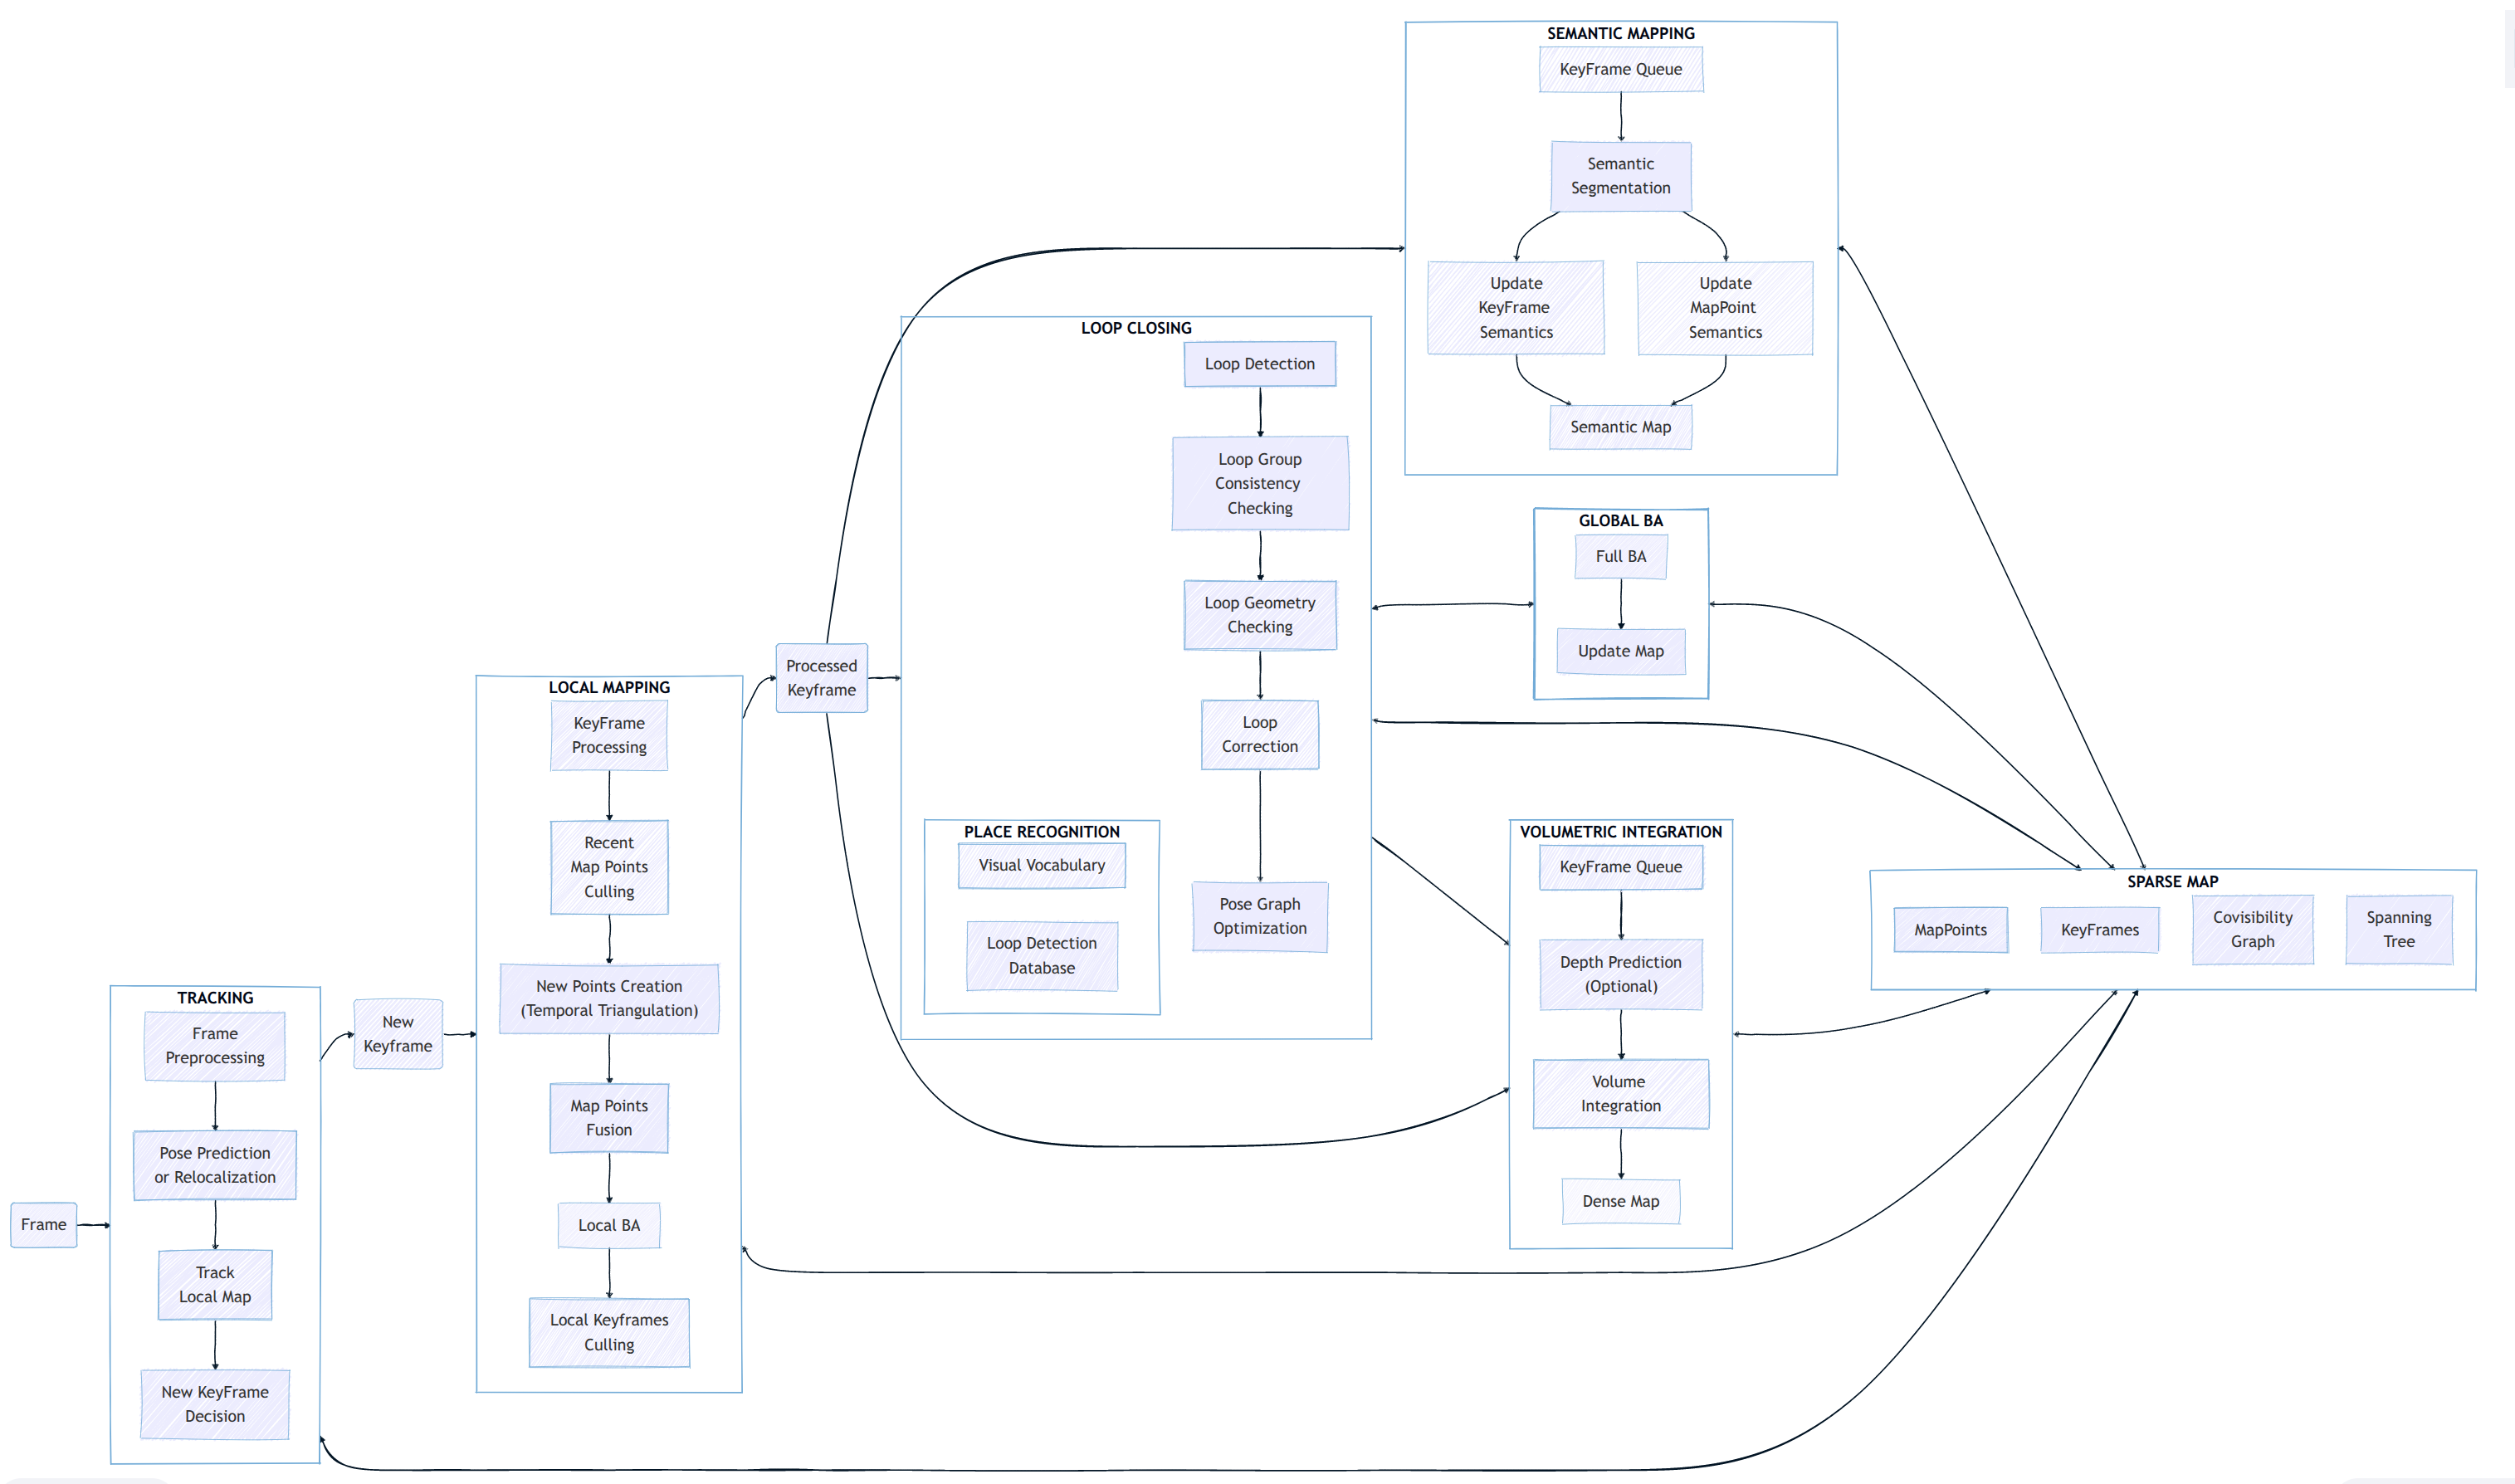
\includegraphics[width=\textwidth]{./images/slam_workflow.png}
\end{center}
\caption{SLAM workflow.}
\label{Fig:SLAMWorfklow}
\end{figure}

\begin{figure}[!t]
\begin{center}
    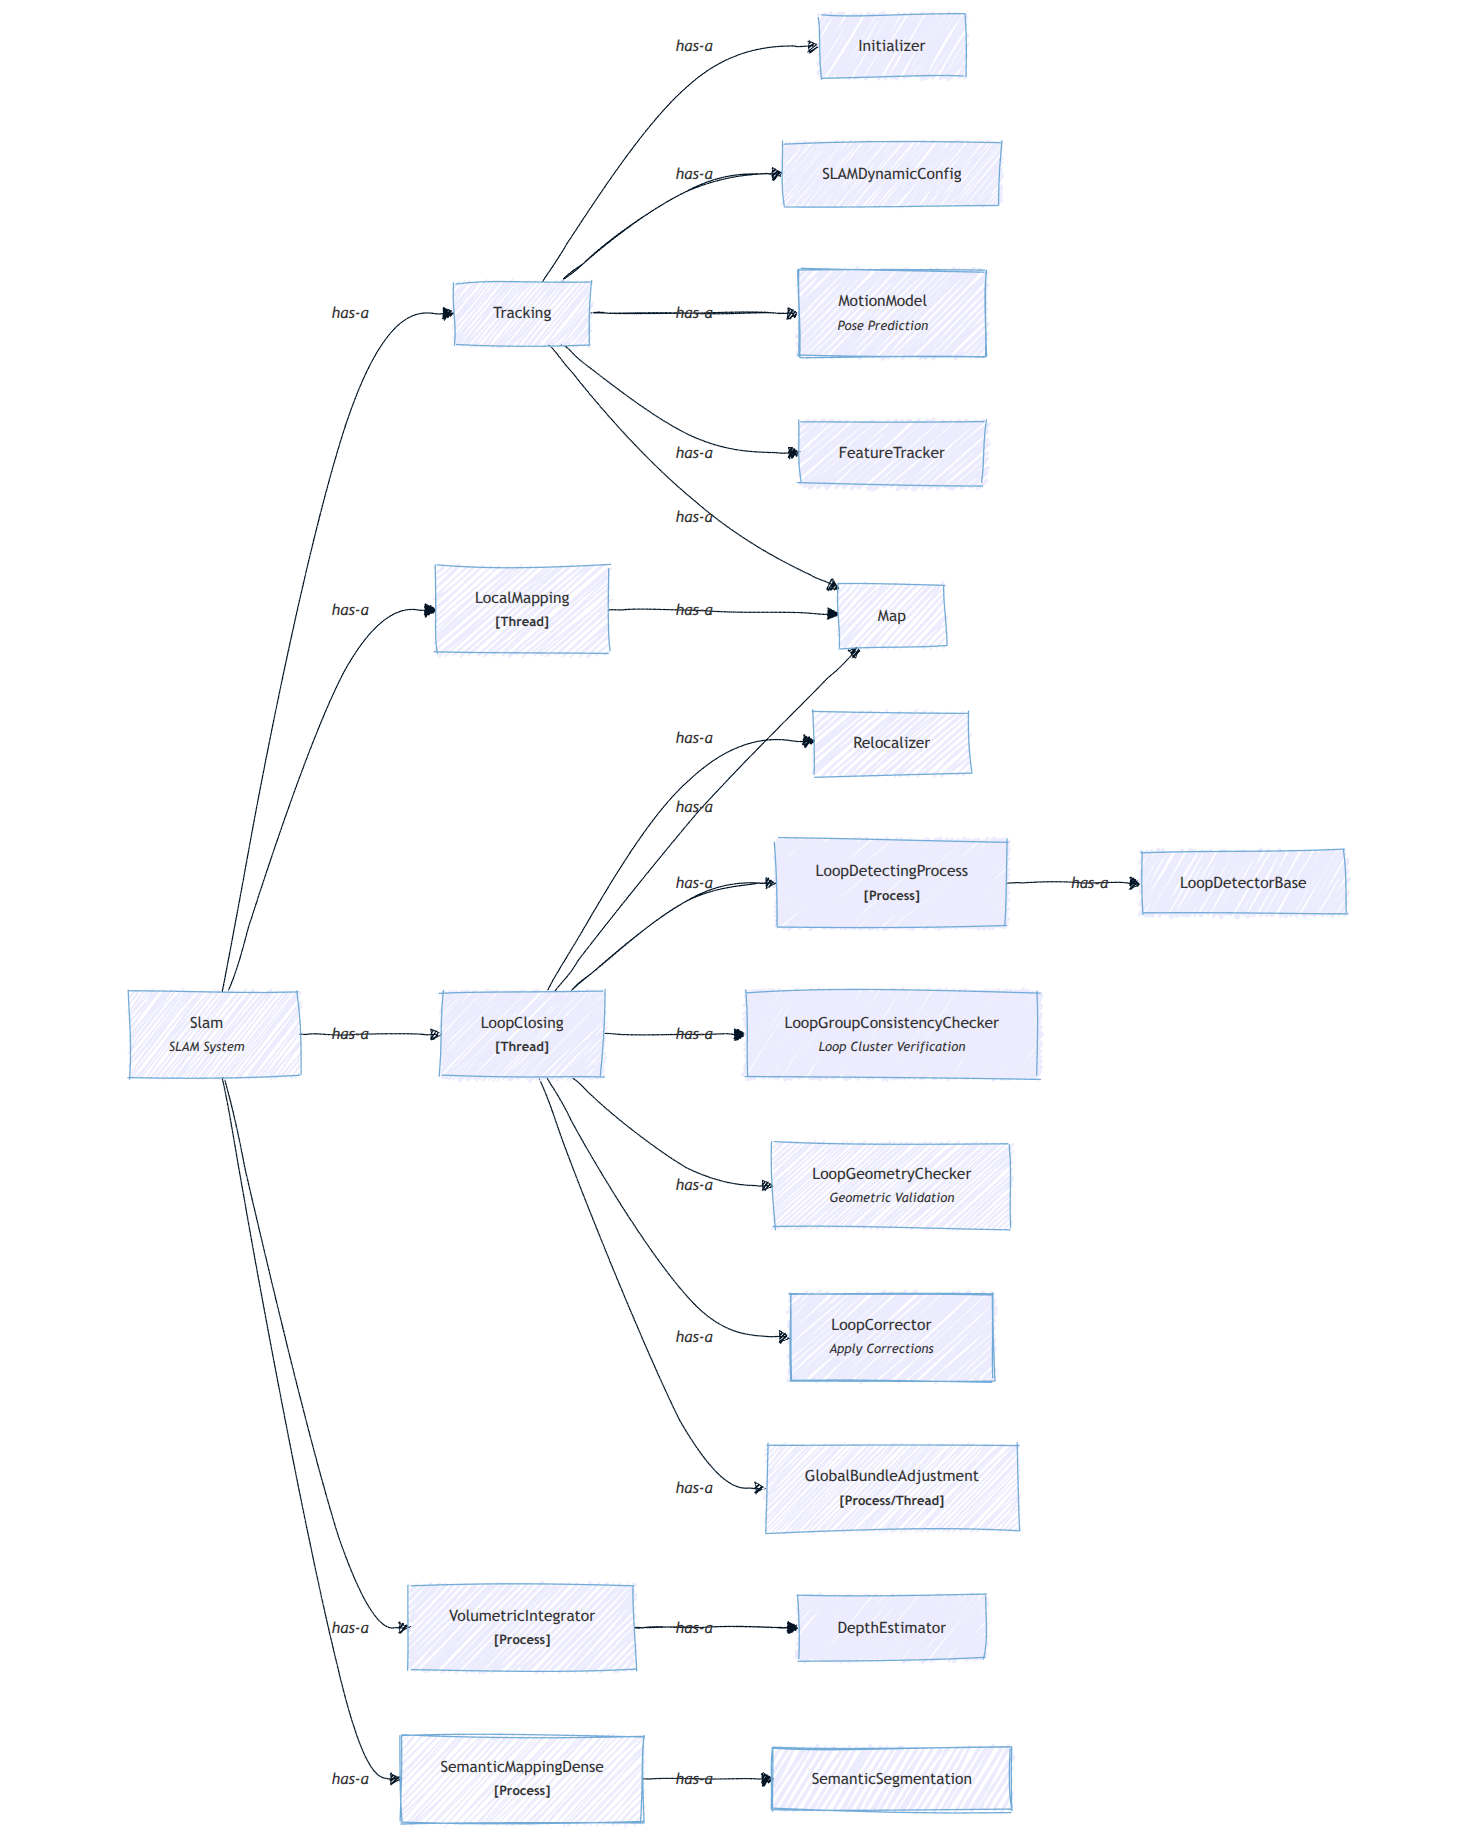
\includegraphics[width=\textwidth]{./images/slam_components.png}
\end{center}
\caption{SLAM components.}
\label{Fig:SLAMComponents}
\end{figure}

\subsection{System overview}\label{system_overview}

This section presents some diagram sketches that provide an overview of the main workflow, system components, and class relationships/dependencies. To make the diagrams more readable, some minor components and arrows have been omitted.


\subsubsection{SLAM Workflow and Components} 

Fig.~\ref{Fig:SLAMWorfklow} illustrates the SLAM workflow, which is composed of six main parallel processing modules:

\begin{itemize}
\item \textit{Tracking}: estimates the camera pose for each incoming frame by extracting and matching local features to the local map, followed by minimizing the reprojection error through motion-only Bundle Adjustment (BA). It includes components such as pose prediction (or relocalization), feature tracking, local map tracking, and keyframe decision-making.
\item \textit{Local Mapping}: updates and refines the local map by processing new keyframes. This involves culling redundant map points, creating new points via temporal triangulation, fusing nearby map points, performing Local BA, and pruning redundant local keyframes.
\item \textit{Loop Closing}: detects and validates loop closures to correct drift accumulated over time. Upon loop detection, it performs loop group consistency checks and geometric verification, applies corrections, and then launches Pose Graph Optimization (PGO) followed by a full Global Bundle Adjustment (GBA). Loop detection itself is delegated to a parallel process, the \textit{Loop Detector}, which operates independently for better responsiveness and concurrency.
\item \textit{Global Bundle Adjustment}: triggered by the Loop Closing module after PGO, this step globally optimizes the trajectory and the sparse structure of the map to ensure consistency across the entire sequence.
\item \textit{Volumetric Integration}: uses the keyframes, with their estimated poses and back-projected point clouds, to reconstruct a dense 3D map of the environment. This module optionally integrates predicted depth maps and maintains a volumetric representation such as a TSDF~\cite{dong2022ash} or incremental Gaussian Splatting-based volume~\cite{matsuki2023gaussian,kerbl20233d}.
\item \textit{Semantic Mapping}: enriches the SLAM map with dense semantic information by applying pixel-wise segmentation to selected keyframes. Semantic predictions are fused across views to assign semantic labels or descriptors to keyframes and map points. The module operates in parallel, consuming keyframes and associated image data from a queue, applying a configured semantic segmentation model, and updating the map with fused semantic features. This enables advanced downstream tasks such as semantic navigation, scene understanding, and category-level mapping.
\end{itemize}

The first four modules follow the established PTAM~\cite{PTAM} and ORB-SLAM~\cite{ORB_SLAM2} paradigm. Here, the \textit{Tracking} module serves as the front-end, while the remaining modules operate as part of the back-end.

In parallel, the system constructs two types of maps:
\begin{itemize}
\item a \emph{sparse map} ${\cal M}_s = ({\cal K}, {\cal P})$, composed of a set of keyframes $\cal K$ and 3D points ${\cal P}$ derived from matched features;
\item a \emph{volumetric map} (or dense map) ${\cal M}_v$, constructed by the Volumetric Integration module, which fuses back-projected point clouds from the keyframes $\cal K$ into a dense 3D model.
\end{itemize}

To ensure consistency between the sparse and volumetric representations, the volumetric map is updated or re-integrated whenever global pose adjustments occur (e.g., after loop closures).

Fig.~\ref{Fig:SLAMComponents} details the internal components and interactions of the above modules. In certain cases, \textbf{processes} are employed instead of \textbf{threads}. This is due to Python's Global Interpreter Lock (GIL), which prevents concurrent execution of multiple threads in a single process. The use of multiprocessing circumvents this limitation, enabling true parallelism at the cost of some inter-process communication overhead (e.g., via pickling). For an insightful discussion, see this related \href{https://www.theserverside.com/blog/Coffee-Talk-Java-News-Stories-and-Opinions/Is-Pythons-GIL-the-software-worlds-biggest-blunder}{post}.



\subsection{Main System Components}

\begin{figure}[!h]
\begin{center}
    \includegraphics[width=0.8\textwidth]{./images/feature_tracker.png}
\end{center}
\caption{Feature tracker.}
\label{Fig:FeatureTracker}
\end{figure}

\subsubsection{Feature Tracker}

The \textit{Feature Tracker} consists of the following key sub-components:

\begin{itemize} 
\item \textit{Feature Manager}: Manages local feature operations. It includes the \texttt{FeatureDetector}, \texttt{FeatureDescriptor}, and adaptors for pyramid management and image tiling. 
\begin{itemize}
\item \textit{Feature Detector}: Identifies salient and repeatable keypoints in the image, such as corners or blobs, which are likely to be robust under viewpoint and illumination changes. 

\item \textit{Feature Descriptor}: Computes a distinctive descriptor for each detected keypoint, encoding its local appearance to enable robust matching across frames. Examples include ORB~\cite{rublee2011orb}, SIFT~\cite{lowe1999object}, or SuperPoint~\cite{detone18superpoint} descriptors.

\end{itemize}

\item \textit{Feature Matcher}: Establishes correspondences between features in successive frames (or stereo pairs) by comparing their descriptors or directly inferring matches from image content. Matching can be performed using brute-force, k-NN with ratio test, or learned matching strategies. Refere to Sect.~\ref{Sect:FeatureMatcher} for futher details.
\end{itemize}

Sect.~\ref{supported-local-features} reports the list of supported local feature extractors and detectors.

The diagram in Fig.~\ref{Fig:FeatureTracker} presents the architecture of the \textit{Feature Tracker} system. It is structured around a \texttt{feature\_tracker\_factory}, which instantiates specific tracker types such as \texttt{LK}, \texttt{DES\_BF}, \texttt{DES\_FLANN}, \texttt{XFEAT}, \texttt{LIGHTGLUE}, and \texttt{LOFTR}. Each tracker type creates a corresponding implementation (e.g., \texttt{LKFeatureTracker}, \texttt{DescriptorFeatureTracker}, etc.), all of which inherit from a common \texttt{FeatureTracker} interface.

The \texttt{FeatureTracker} class is composed of several key sub-components, including a \texttt{FeatureManager}, \texttt{FeatureDetector}, \texttt{FeatureDescriptor}, \texttt{PyramidAdaptor}, \texttt{BlockAdaptor}, and \texttt{FeatureMatcher}. The \texttt{FeatureManager} itself also encapsulates instances of the detector, descriptor, and adaptors, highlighting the modular and reusable design of the tracking pipeline.


\begin{figure}[!t]
\begin{center}
    \includegraphics[width=0.8\textwidth]{./images/feature_matcher.png}
\end{center}
\caption{Feature matcher.}
\label{Fig:FeatureMatcher}
\end{figure}

\begin{figure}[!t]
\begin{center}
    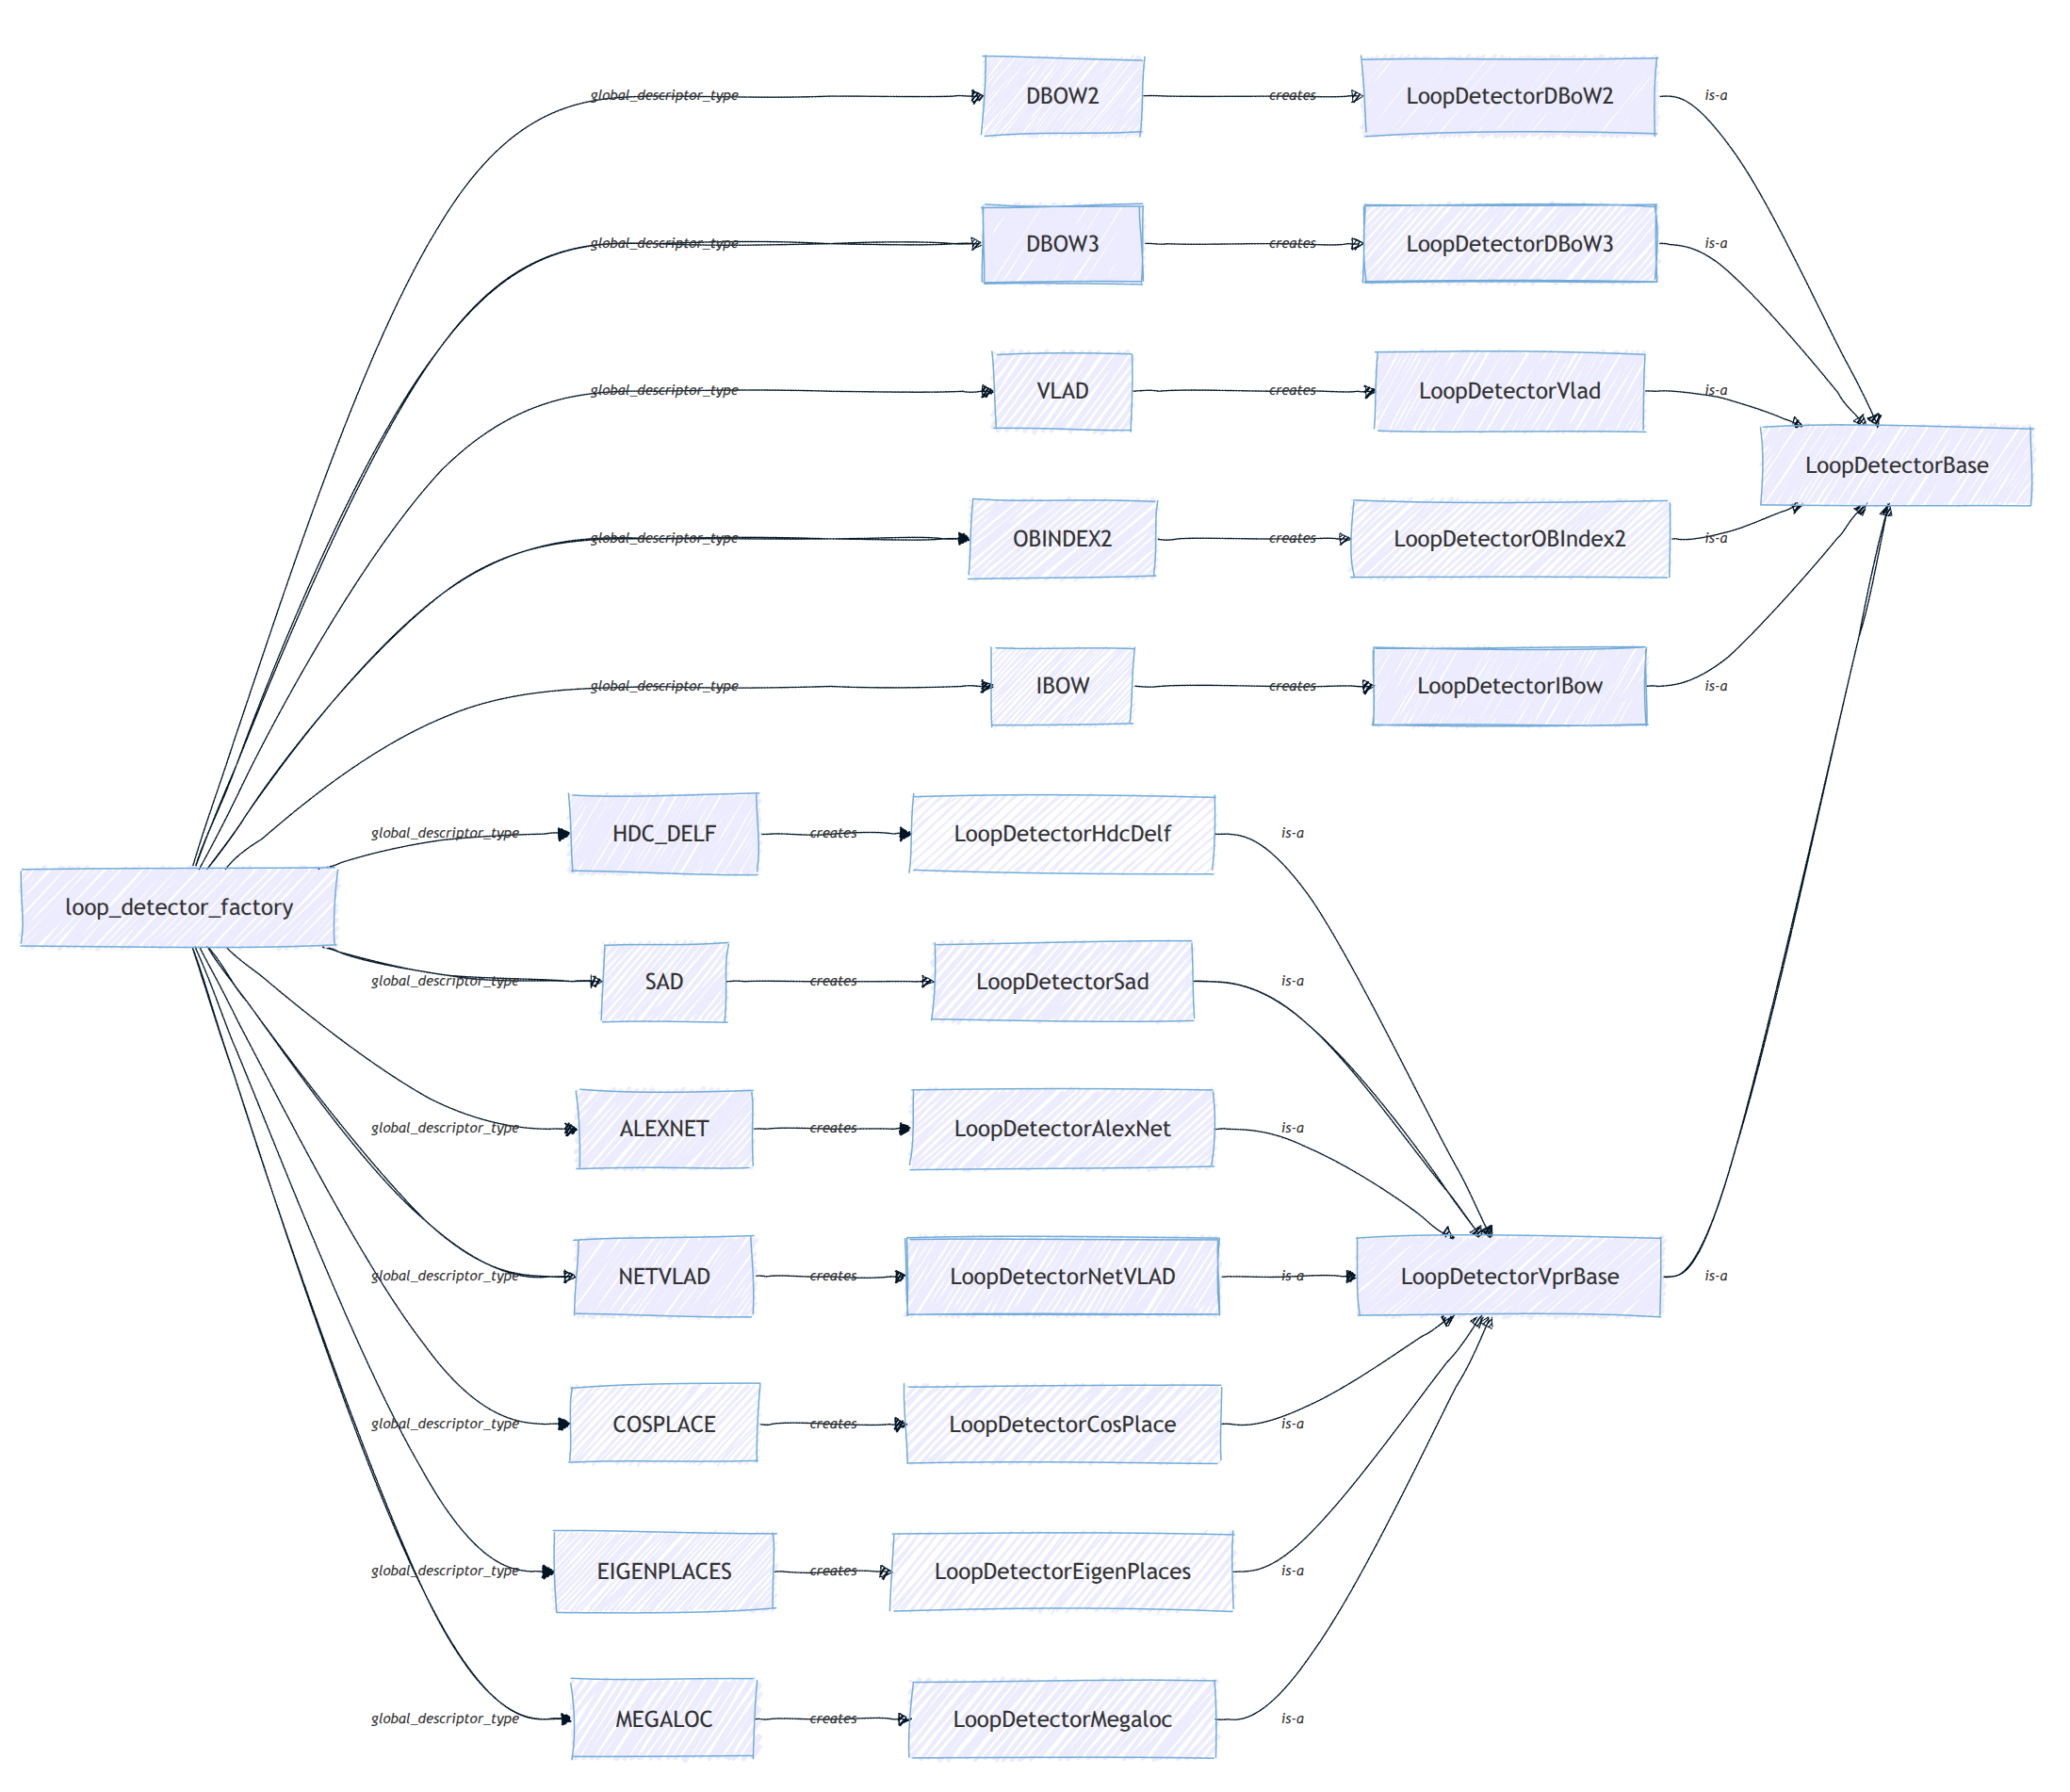
\includegraphics[width=0.7\textwidth]{./images/loop_detector.png}
\end{center}
\caption{Loop detector.}
\label{Fig:LoopDetector}
\end{figure}


\subsubsection{Feature Matcher}\label{Sect:FeatureMatcher}

The diagram in Fig.~\ref{Fig:FeatureMatcher} illustrates the architecture of the \textit{Feature Matcher} module. At its core is the \texttt{feature\_matcher\_factory}, which instantiates matchers based on a specified \texttt{matcher\_type}, such as \texttt{BF}, \texttt{FLANN}, \texttt{XFEAT}, \texttt{LIGHTGLUE}, and \texttt{LOFTR}. Each of these creates a corresponding matcher implementation (e.g., \texttt{BfFeatureMatcher}, \texttt{FlannFeatureMatcher}, etc.), all inheriting from a common \texttt{FeatureMatcher} interface.

The \texttt{FeatureMatcher} class encapsulates several configuration parameters and components, including the matcher engine (\texttt{cv2.BFMatcher}, \texttt{FlannBasedMatcher}, \texttt{xfeat.XFeat}, etc.), as well as the \texttt{matcher\_type}, \texttt{detector\_type}, \texttt{descriptor\_type}, \texttt{norm\_type}, and \texttt{ratio\_test} fields. This modular structure supports extensibility and facilitates switching between traditional and learning-based feature matching backends.

The Section~\ref{supported-matchers} reports a list of supported feature matchers. 


\begin{figure}[!t]
\begin{center}
    \includegraphics[width=\textwidth]{./images/depth_estimator.png}
\end{center}
\caption{Depth estimator.}
\label{Fig:DepthEstimator}
\end{figure}


\subsubsection{Loop Detector}

The diagram in Fig.~\ref{Fig:LoopDetector} shows the architecture of the \textit{Loop Detector} component. A central \texttt{loop\_detector\_factory} instantiates loop detectors based on the selected \texttt{global\_descriptor\_type}, which may include traditional descriptors (e.g., \texttt{DBOW2}, \texttt{VLAD}, \texttt{IBOW}) or deep learning-based embeddings (e.g., \texttt{NetVLAD}, \texttt{CosPlace}, \texttt{EigenPlaces}).

Each descriptor type creates a corresponding loop detector implementation (e.g., \texttt{LoopDetectorDBoW2}, \texttt{LoopDetectorNetVLAD}), all of which inherit from a base class hierarchy. Traditional methods inherit directly from \texttt{LoopDetectorBase}, while deep learning-based approaches inherit from \texttt{LoopDetectorVprBase}, which itself extends \texttt{LoopDetectorBase}. This design supports modular integration of diverse place recognition techniques within a unified loop closure framework.

The Section~\ref{supported-global-descriptors-and-local-descriptor-aggregation-methods} reports a list of supported loop closure methods with the adopted global descriptors and local descriptor aggregation methods.


\subsubsection{Depth Estimator}

The diagram in Fig.~\ref{Fig:DepthEstimator} illustrates the architecture of the \textit{Depth Estimator} module. A central \texttt{depth\_estimator\_factory} creates instances of various depth estimation backends based on the selected \texttt{depth\_estimator\_type}, including both traditional and learning-based methods such as \texttt{DEPTH\_SGBM}, \texttt{DEPTH\_RAFT\_STEREO}, \texttt{DEPTH\_ANYTHING\_V2}, \texttt{DEPTH\_MAST3R}, and \texttt{DEPTH\_MVDUST3R}.

Each estimator type instantiates a corresponding implementation (e.g., \texttt{DepthEstimatorSgbm}, \texttt{DepthEstimatorCrestereo}, etc.), all inheriting from a common \texttt{DepthEstimator} interface. This base class encapsulates shared dependencies such as the \texttt{camera}, \texttt{device}, and \texttt{model} components, allowing for modular integration of heterogeneous depth estimation techniques across stereo, monocular, and multi-view pipelines.

The Section~\ref{supported-depth-prediction-models} reports a list of supported depth estimation/prediction models.

\begin{figure}[!t]
\begin{center}
    \includegraphics[width=\textwidth]{./images/volumetric_integrator.png}
\end{center}
\caption{Volumetric integrator.}
\label{Fig:VolumetricIntegrator}
\end{figure}

\subsubsection{Volumetric Integrator}

The diagram in Fig.~\ref{Fig:VolumetricIntegrator} illustrates the structure of the \textit{Volumetric Integrator} module. At its core, the \texttt{volumetric\_integrator\_factory} generates specific volumetric integrator instances based on the selected \texttt{volumetric\_integrator\_type}, such as \texttt{TSDF} and \texttt{GAUSSIAN\_SPLATTING}.

Each type instantiates a dedicated implementation (e.g., \texttt{VolumetricIntegratorTSDF}, \texttt{VolumetricIntegrator\-Gaussian\-Splatting}), which inherits from a common \texttt{VolumetricIntegratorBase}. This base class encapsulates key components including the \texttt{camera}, a \texttt{keyframe\_queue}, and the \texttt{volume}, enabling flexible integration of various 3D reconstruction methods within a unified pipeline.

The Section~\ref{supported-volumetric-mapping-methods} reports a list of supported volume integration methods.


\begin{figure}[!t]
\begin{center}
    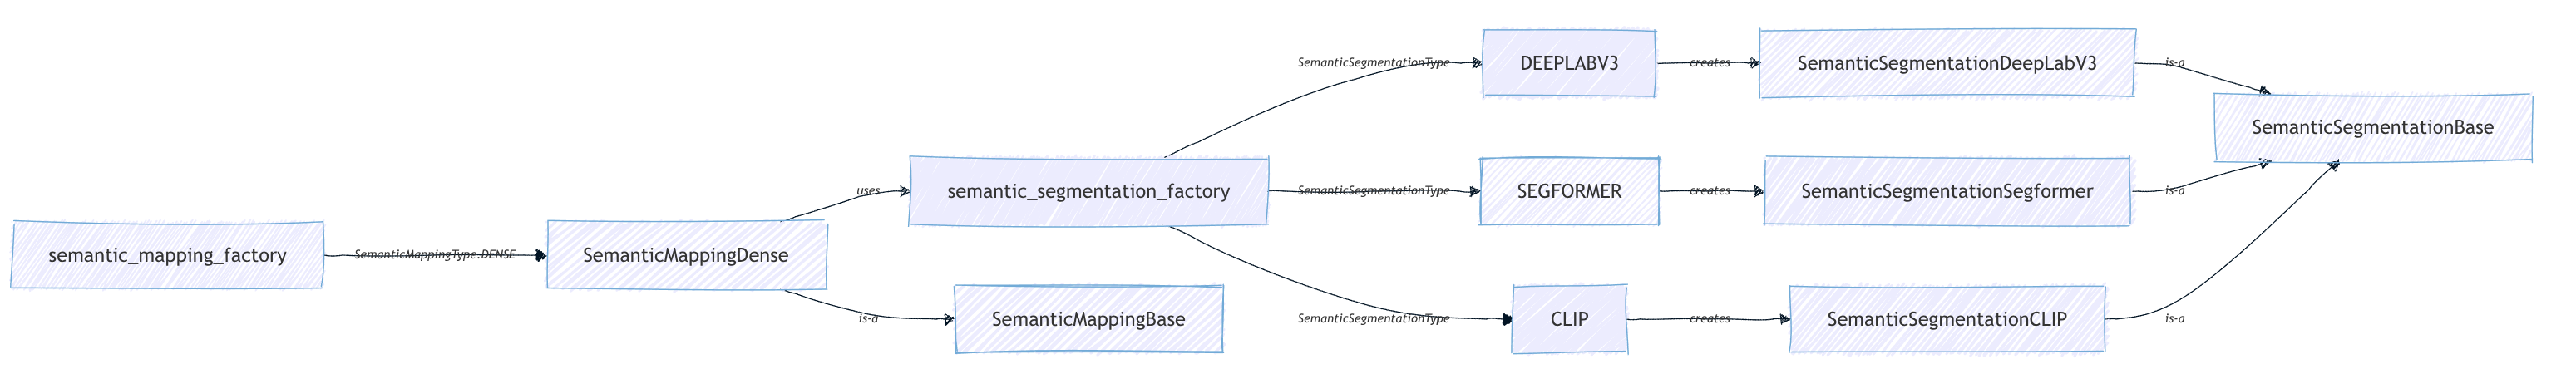
\includegraphics[width=\textwidth]{./images/semantic_mapping.png}
\end{center}
\caption{Semantic Mapping.}
\label{Fig:SemanticMapping}
\end{figure}



\subsubsection{Semantic Mapping}

The diagram in Fig.~\ref{Fig:SemanticMapping} outlines the architecture of the \textit{Semantic Mapping} module. At its core is the \texttt{semantic\_mapping\_factory}, which creates semantic mapping instances according to the selected \texttt{semantic\_mapping\_type}. Currently, the supported type is \texttt{DENSE}, which instantiates the \texttt{SemanticMappingDense} class. This class extends \texttt{SemanticMappingBase} and runs asynchronously in a dedicated thread to process keyframes as they become available.

\texttt{SemanticMappingDense} integrates semantic information into the SLAM map by leveraging per-frame predictions from a semantic segmentation model. The segmentation model is instantiated via the \texttt{semantic\_segmentation\_factory}, based on the selected \texttt{semantic\_segmentation\_type}. Supported segmentation backends include \texttt{DEEPLABV3}, \texttt{SEGFORMER}, and \texttt{CLIP}, each of which corresponds to a dedicated class (\texttt{SemanticSegmentationDeepLabV3}, \texttt{SemanticSegmentationSegformer}, \texttt{SemanticSegmentationCLIP}) inheriting from the shared \texttt{SemanticSegmentationBase}.

The system supports multiple semantic feature representations~--~such as categorical labels, probability vectors, and high-dimensional feature embeddings~--~and fuses them into the map using configurable methods like count-based fusion, Bayesian fusion, or feature averaging.

This modular design decouples semantic segmentation from mapping logic, enabling flexible combinations of segmentation models, datasets (e.g., \texttt{NYU40}, \texttt{Cityscapes}), and fusion strategies. It also supports customization via configuration files or programmatic APIs for dataset-specific tuning or deployment.

The Section~\ref{semantic-mapping} provides a list of supported semantic segmentation methods.





%\hypertarget{troubleshooting-and-performance-issues}{%
%\subsection{Troubleshooting and performance
%issues}\label{troubleshooting-and-performance-issues}}
%
%If you run into issues or errors during the installation process or at
%run-time, please, check the
%\href{./docs/TROUBLESHOOTING.md}{docs/TROUBLESHOOTING.md} file. Before
%submitting a new git issue please read
%\href{docs/TROUBLESHOOTING.md\#submitting-a-git-issue}{here}.

%\clearpage
\FloatBarrier

\hypertarget{usage}{%
\section{Usage}\label{usage}}

Open a new terminal and start experimenting with the scripts. In each
new terminal you are supposed to start with this command:

\begin{scriptsize}
\begin{Shaded}
\begin{Highlighting}[]
\NormalTok{$ }\BuiltInTok{.} \ExtensionTok{pyenv-activate.sh}   \CommentTok{#  Activate pyslam python virtual environment. This is only needed once in a new terminal.}
\end{Highlighting}
\end{Shaded}
\end{scriptsize}

The file \href{./config.yaml}{config.yaml} can be used as a unique
entry-point to configure the system and its global configuration
parameters contained in
\href{./config_parameters.py}{config\_parameters.py}. Further
information on how to configure pySLAM are provided
\protect\hyperlink{selecting-a-dataset-and-different-configuration-parameters}{here}.


\hypertarget{visual-odometry}{%
\subsubsection{Visual odometry}\label{visual-odometry}}

The basic \textbf{Visual Odometry} (VO) can be run with the following
commands:

\begin{scriptsize}
\begin{Shaded}
\begin{Highlighting}[]
\NormalTok{$ }\BuiltInTok{.} \ExtensionTok{pyenv-activate.sh}   \CommentTok{#  Activate pyslam python virtual environment. This is only needed once in a new terminal.}
\NormalTok{$ }\ExtensionTok{./main_vo.py}
\end{Highlighting}
\end{Shaded}
\end{scriptsize}


By default, this processes a
\href{http://www.cvlibs.net/datasets/kitti/eval_odometry.php}{KITTI}
video (available in the folder \texttt{data/videos}) by using its
corresponding camera calibration file (available in the folder
\texttt{settings}), and its groundtruth (available in the same
\texttt{data/videos} folder). If matplotlib windows are used, you can
stop \texttt{main\_vo.py} by focusing/clicking on one of them and
pressing the key `Q'. As explained above, this very \emph{basic} script
\texttt{main\_vo.py} \textbf{strictly requires a ground truth}. Now,
with RGBD datasets, you can also test the \textbf{RGBD odometry} with
the classes \texttt{VisualOdometryRgbd} or
\texttt{VisualOdometryRgbdTensor} (ground truth is not required here).

\hypertarget{full-slam}{%
\subsubsection{Full SLAM}\label{full-slam}}

Similarly, you can test the \textbf{full SLAM} by running
\texttt{main\_slam.py}:\\

\begin{scriptsize}
\begin{Shaded}
\begin{Highlighting}[]
\NormalTok{$ }\BuiltInTok{.} \ExtensionTok{pyenv-activate.sh}   \CommentTok{#  Activate pyslam python virtual environment. This is only needed once in a new terminal.}
\NormalTok{$ }\ExtensionTok{./main_slam.py}
\end{Highlighting}
\end{Shaded}
\end{scriptsize}

This will process the same default
\href{(http://www.cvlibs.net/datasets/kitti/eval_odometry.php)}{KITTI}
video (available in the folder \texttt{data/videos}) by using its
corresponding camera calibration file (available in the folder
\texttt{settings}). You can stop it by focusing/clicking on one of the
opened windows and pressing the key `Q' or closing the 3D pangolin GUI.
\hypertarget{selecting-a-dataset-and-different-configuration-parameters}{%
\subsubsection{Selecting a dataset and different configuration
parameters}\label{selecting-a-dataset-and-different-configuration-parameters}}

The file \href{./config.yaml}{config.yaml} can be used as a unique
entry-point to configure the system, the target dataset and its global
configuration parameters set in
\href{./config_parameters.py}{config\_parameters.py}.
To process a different \textbf{dataset} with both VO and SLAM scripts,
you need to update the file \href{./config.yaml}{config.yaml}:
\begin{itemize}
\item Select
your dataset \texttt{type} in the section \texttt{DATASET} (further
details in the section \emph{\protect\hyperlink{datasets}{Datasets}}
below for further details). This identifies a corresponding dataset
section (e.g.~\texttt{KITTI\_DATASET}, \texttt{TUM\_DATASET}, etc). 
\item  Select the \texttt{sensor\_type} (\texttt{mono}, \texttt{stereo},
\texttt{rgbd}) in the chosen dataset section.
\item  Select the camera \texttt{settings} file in the dataset section
(further details in the section
\emph{\protect\hyperlink{camera-settings}{Camera Settings}} below).
\item Set the \texttt{groudtruth\_file} accordingly. Further details in the
section \emph{\protect\hyperlink{datasets}{Datasets}} below (see also
the files \texttt{io/ground\_truth.py},
\texttt{io/convert\_groundtruth\_to\_simple.py}).
\end{itemize}

You can use the section \texttt{GLOBAL\_PARAMETERS} of the file
\href{./config.yaml}{config.yaml} to override the global configuration
parameters set in \href{./config_parameters.py}{config\_parameters.py}.
This is particularly useful when running a
\protect\hyperlink{evaluating-slam}{SLAM evaluation}.

\hypertarget{feature-tracking}{%
\subsection{Feature tracking}\label{feature-tracking}}

If you just want to test the basic feature tracking capabilities
(\emph{feature detector} + \emph{feature descriptor} + \emph{feature
matcher}) and get a taste of the different available local features, run \\

\begin{scriptsize}
\begin{Shaded}
\begin{Highlighting}[]
\NormalTok{$ }\BuiltInTok{.} \ExtensionTok{pyenv-activate.sh}   \CommentTok{#  Activate pyslam python virtual environment. This is only needed once in a new terminal.}
\NormalTok{$}\ExtensionTok{./main_feature_matching.py}
\end{Highlighting}
\end{Shaded}
\end{scriptsize}


In any of the above scripts, you can choose any detector/descriptor
among \emph{ORB}, \emph{SIFT}, \emph{SURF}, \emph{BRISK}, \emph{AKAZE},
\emph{SuperPoint}, etc. (see the section
\emph{\protect\hyperlink{supported-local-features}{Supported Local
Features}} below for further information).

Some basic examples are available in the subfolder
\texttt{test/cv}. In particular, as for feature
detection/description, you may want to take a look at
\href{./test/cv/test_feature_manager.py}{test/cv/test\_feature\_manager.py}
too.

\hypertarget{loop-closing}{%
\subsection{Loop closing}\label{loop-closing}}

Many \protect\hyperlink{loop-closing}{loop closing methods} are
available, combining different
\protect\hyperlink{local-descriptor-aggregation-methods}{aggregation
methods} and \protect\hyperlink{global-descriptors}{global descriptors}.

While running full SLAM, loop closing is enabled by default and can be
disabled by setting \texttt{kUseLoopClosing=False} in
\texttt{config\_parameters.py}. Different configuration options
\texttt{LoopDetectorConfigs} can be found in
\url{loop_closing/loop_detector_configs.py}: Code comments provide
additional useful details.

One can start experimenting with loop closing methods by using the
examples in \texttt{test/loopclosing}. The example
\href{./test/loopclosing/test_loop_detector.py}{test/loopclosing/test\_loop\_detector.py}
is the recommended entry point.

\hypertarget{vocabulary-management}{%
\paragraph{Vocabulary management}\label{vocabulary-management}}

\texttt{DBoW2}, \texttt{DBoW3}, and \texttt{VLAD} require
\textbf{pre-trained vocabularies}. ORB-based vocabularies are
automatically downloaded in the \texttt{data} folder (see
\url{loop_closing/loop_detector_configs.py}).

To create a new vocabulary, follow these steps:

\begin{enumerate}
\def\labelenumi{\arabic{enumi}.}
\item
  \textbf{Generate an array of descriptors}: Use the script \\
  \texttt{test/loopclosing/test\_gen\_des\_array\_from\_imgs.py} to
  generate the array of descriptors that will be used to train the new
  vocabulary. Select your desired descriptor type via the tracker
  configuration.
\item
  \textbf{DBOW vocabulary generation}: Train your target DBOW vocabulary
  by using the script
  \texttt{test/loopclosing/test\_gen\_dbow\_voc\_from\_des\_array.py}.
\item
  \textbf{VLAD vocabulary generation}: Train your target VLAD
  ``vocabulary'' by using the script
  \texttt{test/loopclosing/test\_gen\_vlad\_voc\_from\_des\_array.py}.
\end{enumerate}

Once you have trained the vocabulary, you can add it in
\url{loop_closing/loop_detector_vocabulary.py} and correspondingly
create a new loop detector configuration in
\url{loop_closing/loop_detector_configs.py} that uses it.

\hypertarget{vocabulary-free-loop-closing}{%
\paragraph{Vocabulary-free loop
closing}\label{vocabulary-free-loop-closing}}

Most methods do not require pre-trained vocabularies. Specifically:
\begin{itemize}
\item \texttt{iBoW} and \texttt{OBindex2}: These methods incrementally build
bags of binary words and, if needed, convert (front-end) non-binary
descriptors into binary ones. 
\item Others: Methods like \texttt{HDC\_DELF},
\texttt{SAD}, \texttt{AlexNet}, \texttt{NetVLAD}, \texttt{CosPlace}, and
\texttt{EigenPlaces} directly extract their specific \textbf{global
descriptors} and process them using dedicated aggregators, independently
from the used front-end descriptors.
\end{itemize}

As mentioned above, only \texttt{DBoW2}, \texttt{DBoW3}, and
\texttt{VLAD} require pre-trained vocabularies.

\hypertarget{double-check-your-loop-detection-configuration-and-verify-vocabulary-compability}{%
\paragraph{Double-check your loop detection configuration and verify
vocabulary
compability}\label{double-check-your-loop-detection-configuration-and-verify-vocabulary-compability}}

\hypertarget{loop-detection-method-based-on-a-pre-trained-vocabulary}{%
\subparagraph{Loop detection method based on a pre-trained
vocabulary}\label{loop-detection-method-based-on-a-pre-trained-vocabulary}}

When selecting a \textbf{loop detection method based on a pre-trained
vocabulary} (such as \texttt{DBoW2}, \texttt{DBoW3}, and \texttt{VLAD}),
ensure the following: 
\begin{enumerate}
\item The back-end and the front-end are using the
same descriptor type (this is also automatically checked for
consistency) or their descriptor managers are independent (see further
details in the configuration options \texttt{LoopDetectorConfigs}
available in \url{loop_closing/loop_detector_configs.py}). 
\item A corresponding pre-trained vocubulary is available. For more details,
refer to the \protect\hyperlink{vocabulary-management}{vocabulary
management section}.
\end{enumerate}

\hypertarget{missing-vocabulary-for-the-selected-front-end-descriptor-type}{%
\subparagraph{Missing vocabulary for the selected front-end descriptor
type}\label{missing-vocabulary-for-the-selected-front-end-descriptor-type}}

If you lack a compatible vocabulary for the selected front-end
descriptor type, you can follow one of these options:\\
1. Create and load the vocabulary (refer to the
\protect\hyperlink{vocabulary-management}{vocabulary management
section}).\\
2. Choose an \texttt{*\_INDEPENDENT} loop detector method, which works
with an independent local\_feature\_manager.\\
3. Select a vocabular-free loop closing method.

See the file \url{loop_closing/loop_detector_configs.py} for further
details.

\hypertarget{volumetric-reconstruction}{%
\subsection{Volumetric reconstruction}\label{volumetric-reconstruction}}

\hypertarget{dense-reconstruction-while-running-slam}{%
\paragraph{Dense reconstruction while running
SLAM}\label{dense-reconstruction-while-running-slam}}

The SLAM back-end hosts a volumetric reconstruction pipeline. This is
disabled by default. You can enable it by setting
\texttt{kUseVolumetricIntegration=True} and selecting your preferred
method \texttt{kVolumetricIntegrationType} in
\texttt{config\_parameters.py}. At present, two methods are available:
\texttt{TSDF} and \texttt{GAUSSIAN\_SPLATTING} (see
\url{dense/volumetric_integrator_factory.py}). Note that you need CUDA
in order to run \texttt{GAUSSIAN\_SPLATTING} method.

At present, the volumetric reconstruction pipeline works with:
\begin{itemize}
\item RGBD datasets 
\item When a \protect\hyperlink{depth-prediction}{depth estimator}
is used
\begin{itemize}
\item[$\circ$] in the back-end with STEREO datasets (you can't use depth
prediction in the back-end with MONOCULAR datasets, further details
\protect\hyperlink{depth-prediction}{here}) 
\item[$\circ$] in the front-end (to emulate an RGBD sensor) and a depth prediction/estimation gets available
for each processed keyframe.
\end{itemize}
\end{itemize}

If you want a mesh as output then set
\texttt{kVolumetricIntegrationExtractMesh=True} in
\texttt{config\_parameters.py}.

\hypertarget{reload-a-saved-sparse-map-and-perform-dense-reconstruction}{%
\paragraph{Reload a saved sparse map and perform dense
reconstruction}\label{reload-a-saved-sparse-map-and-perform-dense-reconstruction}}

Use the script \texttt{main\_map\_dense\_reconstruction.py} to reload a
saved sparse map and to perform dense reconstruction by using its posed
keyframes as input. You can select your preferred dense reconstruction
method directly in the script.

\begin{itemize}
\tightlist
\item
  To check what the volumetric integrator is doing, run in another shell
  \texttt{tail\ -f\ logs/volumetric\_integrator.log} (from repository
  root folder).
\item
  To save the obtained dense and sparse maps, press the \texttt{Save}
  button on the GUI.
\end{itemize}

\hypertarget{reload-and-check-your-dense-reconstruction}{%
\paragraph{Reload and check your dense
reconstruction}\label{reload-and-check-your-dense-reconstruction}}

You can check the output pointcloud/mesh by using
\href{https://www.cloudcompare.org/}{CloudCompare}.

In the case of a saved Gaussian splatting model, you can visualize it
by: 
\begin{enumerate}
\item Using the
\href{https://playcanvas.com/supersplat/editor}{superslat editor} (drag
and drop the saved Gaussian splatting \texttt{.ply} pointcloud in the
editor interface). 

\item Getting into the folder
\texttt{test/gaussian\_splatting} and running:\\
%\begin{scriptsize}
%\begin{Shaded}
%\begin{Highlighting}[]
%\NormalTok{$ }\BuiltInTok{\ExtensionTok{python\ test\_gsm.py\ -\/-load\ \textless{}gs\_checkpoint\_path\textgreater{}}}   
%\end{Highlighting}
%\end{Shaded}
%\end{scriptsize}
\begin{codeblock}
\codeline{python\ test\_gsm.py\ -\/-load\ \textless{}gs\_checkpoint\_path\textgreater{}}
\end{codeblock}

The \texttt{<gs\_checkpoint\_path>} is expected to have the following structure:\\
\begin{scriptsize}
\begin{Shaded}
\begin{Highlighting}[]
\NormalTok{+-- gs_checkpoint_path}
\NormalTok{|   +-- pointcloud         \textit{# folder containing different subfolders, each one with a saved .ply}}
\NormalTok{|                          \textit{# encoding the gaussian splatting model at a specific iteration/checkpoint}}
\NormalTok{|   +-- last_camera.json}
\NormalTok{|   +-- config.yml}
\end{Highlighting}
\end{Shaded}
\end{scriptsize}

\end{enumerate}



\hypertarget{controlling-the-spatial-distribution-of-keyframe-fov-centers}{%
\paragraph{Controlling the spatial distribution of keyframe FOV
centers}\label{controlling-the-spatial-distribution-of-keyframe-fov-centers}}

If you are targeting volumetric reconstruction while running SLAM, you
can enable a \textbf{keyframe generation policy} designed to manage the
spatial distribution of keyframe field-of-view (FOV) centers. The
\emph{FOV center of a camera} is defined as the backprojection of its
image center, calculated using the median depth of the frame. With this
policy, a new keyframe is generated only if its FOV center is farther
than a predefined distance from the nearest existing keyframe's FOV
center. You can enable this policy by setting the following parameters
in the yaml setting:\\

\begin{scriptsize}
\begin{Shaded}
\begin{Highlighting}[]
\FunctionTok{KeyFrame.useFovCentersBasedGeneration:}\AttributeTok{ }\DecValTok{1}\AttributeTok{  }\CommentTok{# compute 3D fov centers of camera frames by using median depth }
\FunctionTok{}\AttributeTok{ }\DecValTok{}\AttributeTok{  }\CommentTok{                                       # use their distances to control keyframe generation}
\FunctionTok{KeyFrame.maxFovCentersDistance:}\AttributeTok{ }\FloatTok{0.2}\AttributeTok{       }\CommentTok{# max distance between fov centers in order to generate a keyframe}
\end{Highlighting}
\end{Shaded}
\end{scriptsize}


\hypertarget{depth-prediction}{%
\subsubsection{Depth prediction}\label{depth-prediction}}

The available depth prediction models can be utilized both in the SLAM
back-end and front-end. 
\begin{itemize}
\item \textbf{Back-end}: Depth prediction can be
enabled in the \protect\hyperlink{volumetric-reconstruction}{volumetric
reconstruction} pipeline by setting the parameter
\texttt{kVolumetricIntegrationUseDepthEstimator=True} and selecting your
preferred \texttt{kVolumetricIntegrationDepthEstimatorType} in
\texttt{config\_parameters.py}. 
\item \textbf{Front-end}: Depth prediction
can be enabled in the front-end by setting the parameter
\texttt{kUseDepthEstimatorInFrontEnd} in \texttt{config\_parameters.py}.
This feature estimates depth images from input color images to emulate a
RGBD camera. Please, note this functionality is still
\emph{experimental} at present time {[}WIP{]}.
\end{itemize}

\textbf{Notes}: 
\begin{itemize}
\item In the case of a \textbf{monocular SLAM}, do NOT use
depth prediction in the back-end volumetric integration: The SLAM (fake)
scale will conflict with the absolute metric scale of depth predictions.
With monocular datasets, you can enable depth prediction to run in the
front-end (to emulated an RGBD sensor). 
\item The depth inference may be
very slow (for instance, with DepthPro it takes \textasciitilde{}1s per
image on my machine). Therefore, the resulting volumetric reconstruction
pipeline may be very slow.
\end{itemize}

Refer to the file
\texttt{depth\_estimation/depth\_estimator\_factory.py} for further
details. Both stereo and monocular prediction approaches are supported.
You can test depth prediction/estimation by using the script
\texttt{main\_depth\_prediction.py}.

\begin{center}\rule{0.5\linewidth}{0.5pt}\end{center}

\hypertarget{semantic-mapping}{%
\subsubsection{Semantic mapping}\label{semantic-mapping}}

The semantic mapping pipeline can be enabled by setting the parameter
\texttt{kDoSemanticMapping=True} in \texttt{config\_parameters.py}. The
best way of configuring the semantic mapping module used is to modify it
in \texttt{semantic\_mapping\_configs.py}.

Different semantic mapping methods are available Currently, we support semantic mapping using dense
semantic segmenetation. 
\begin{itemize}
\item \texttt{DEEPLABV3}: from \texttt{torchvision}, pre-trained on COCO/VOC.
\item \texttt{SEGFORMER}: from \texttt{transformers}, pre-trained on Cityscapes or ADE20k.
\item \texttt{CLIP}: from \texttt{f3rm} package for open-vocabulary support.
\end{itemize}
Semantic features are assigned to keypoints on
the image and fused into map points. The semantic features can be: 
\begin{itemize}
\item \textit{Labels}: categorical labels as numbers.
\item \textit{Probability vectors}: probability vectors for each class.
\item \textit{Feature vectors}: feature vectors
obtained from an encoder. This is generally used for open vocabulary
mapping.
\end{itemize}

\begin{center}\rule{0.5\linewidth}{0.5pt}\end{center}

\hypertarget{saving-and-reloading}{%
\subsection{Saving and reloading}\label{saving-and-reloading}}

\hypertarget{save-the-a-map}{%
\subsubsection{Save the a map}\label{save-the-a-map}}

When you run the script \texttt{main\_slam.py}
(\texttt{main\_map\_dense\_reconstruction.py}): 
\begin{itemize}
\item You can save the
current map state by pressing the button \texttt{Save} on the GUI. This
saves the current map along with front-end, and backend configurations
into the default folder \texttt{results/slam\_state}
(\texttt{results/slam\_state\_dense\_reconstruction}). 
\item To change the
default saving path, open \texttt{config.yaml} and update target
\texttt{folder\_path} in the section:
\begin{scriptsize}
\begin{Shaded}
\begin{Highlighting}[]
\ExtensionTok{SYSTEM_STATE}\NormalTok{:}
  \ExtensionTok{folder_path}\NormalTok{: results/slam_state   }\CommentTok{# default folder path (relative to repository root) where the system state is saved or reloaded}
\end{Highlighting}
\end{Shaded}
\end{scriptsize}
\end{itemize}

\hypertarget{reload-a-saved-map-and-relocalize-in-it}{%
\subsubsection{Reload a saved map and relocalize in
it}\label{reload-a-saved-map-and-relocalize-in-it}}

\begin{itemize}
\item
  A saved map can be loaded and visualized in the GUI by running: \\

\begin{scriptsize}
\begin{Shaded}
\begin{Highlighting}[]
\NormalTok{$ }\BuiltInTok{.} \ExtensionTok{pyenv-activate.sh}   \CommentTok{#  Activate pyslam python virtual environment. This is only needed once in a new terminal.}
\NormalTok{$ }\ExtensionTok{./main_map_viewer.py}  \CommentTok{#  Use the --path options to change the input path}
\end{Highlighting}
\end{Shaded}

\end{scriptsize}

\item
  To enable map reloading and relocalization when running
  \texttt{main\_slam.py}, open \texttt{config.yaml} and set \\

\begin{scriptsize}
\begin{Shaded}
\begin{Highlighting}[]
\ExtensionTok{SYSTEM_STATE}\NormalTok{:}
  \ExtensionTok{load_state}\NormalTok{: True                  }\CommentTok{# flag to enable SLAM state reloading (map state + loop closing state)}
  \ExtensionTok{folder_path}\NormalTok{: results/slam_state   }\CommentTok{# default folder path (relative to repository root) where the system state is saved or reloaded}
\end{Highlighting}
\end{Shaded}
\end{scriptsize}

\end{itemize}

Note that pressing the \texttt{Save} button saves the current map,
front-end, and backend configurations. Reloading a saved map overwrites
the current system configurations to ensure descriptor compatibility.

\hypertarget{trajectory-saving}{%
\subsubsection{Trajectory saving}\label{trajectory-saving}}

Estimated trajectories can be saved in three different formats:
\emph{TUM} (The Open Mapping format), \emph{KITTI} (KITTI Odometry
format), and \emph{EuRoC} (EuRoC MAV format). pySLAM saves two
\textbf{types} of trajectory estimates:

\begin{itemize}
\tightlist
\item
  \textbf{Online}: In \emph{online} trajectories, each pose estimate
  depends only on past poses. A pose estimate is saved at the end of
  each front-end iteration on current frame.
\item
  \textbf{Final}: In \emph{final} trajectories, each pose estimate
  depends on both past and future poses. A pose estimate is refined
  multiple times by LBA windows that cover it and by PGO and GBA during
  loop closures.
\end{itemize}

To enable trajectory saving, open \texttt{config.yaml} and search for
the \texttt{SAVE\_TRAJECTORY}: set \texttt{save\_trajectory:\ True},
select your \texttt{format\_type} (\texttt{tum}, \texttt{kitti},
\texttt{euroc}), and the output filename. For instance for a
\texttt{tum} format output: \\

\begin{scriptsize}
\begin{Shaded}
\begin{Highlighting}[]
\ExtensionTok{SAVE_TRAJECTORY}\NormalTok{:}
  \ExtensionTok{save_trajectory}\NormalTok{: True}
  \ExtensionTok{format_type}\NormalTok{: kitti             }\CommentTok{# supported formats: `tum`, `kitti`, `euroc`}
  \ExtensionTok{output_folder}\NormalTok{: results/metrics }\CommentTok{# relative to pyslam root folder }
  \ExtensionTok{basename}\NormalTok{: trajectory           }\CommentTok{# basename of the trajectory saving output}
\end{Highlighting}
\end{Shaded}
\end{scriptsize}

\hypertarget{optimization-engines}{%
\subsubsection{Optimization engines}\label{optimization-engines}}

Currently, pySLAM supports both \texttt{g2o} and \texttt{gtsam} for
graph optimization, with \texttt{g2o} set as the default engine. While
\texttt{gtsam} is fully supported, it remains experimental and a work in
progress. You can enable \texttt{gtsam} by setting to \texttt{True} the
following parameters in \texttt{config\_parameters.py}:

\begin{scriptsize}
  \begin{Shaded}
    \begin{Highlighting}[]
      \CommentTok{# Optimization engine }
    \NormalTok{  kOptimizationFrontEndUseGtsam }\OperatorTok{=} \VariableTok{True}    
    \NormalTok{  kOptimizationBundleAdjustUseGtsam }\OperatorTok{=} \VariableTok{True} 
    \NormalTok{  kOptimizationLoopClosingUseGtsam }\OperatorTok{=} \VariableTok{True} 
    \end{Highlighting}
    \end{Shaded}
\end{scriptsize}

Additionally, the \texttt{gtsam\_factors} package provides custom Python
bindings for features not included in the original gtsam framework. See
\href{./thirdparty/gtsam_factors/README.md}{here} for further details.

\hypertarget{slam-gui}{%
\subsection{SLAM GUI}\label{slam-gui}}

Some quick information about the non-trivial GUI buttons of \texttt{main\_slam.py}:

\begin{itemize}
    \item \texttt{Step}: Enter the \emph{Step by step mode}. Press the button \texttt{Step} a first time to pause. Then, press it again to make the pipeline process a single new frame.

    \item \texttt{Save}: Save the map into the file \texttt{map.json}. You can visualize it back by using the script \texttt{main\_map\_viewer.py} (as explained above).

    \item \texttt{Reset}: Reset SLAM system.

    \item \texttt{Draw Ground Truth}: If a ground truth dataset (e.g., KITTI,
    TUM, EUROC, or REPLICA) is loaded, you can visualize it by pressing this
    button. The ground truth trajectory will be displayed in 3D and will be
    progressively aligned with the estimated trajectory, updating
    approximately every 10-30 frames. As more frames are processed, the
    alignment between the ground truth and estimated trajectory becomes more
    accurate. After about 20 frames, if the button is pressed, a window will
    appear showing the Cartesian alignment errors along the main axes (i.e.,
    $e_x, e_y, e_z$ and the history of the total $RMSE$ between
    the ground truth and the aligned estimated trajectories.
\end{itemize}

\hypertarget{monitor-the-logs-for-tracking-local-mapping-and-loop-closing-simultaneously}{%
\subsection{Monitor the logs for tracking, local mapping, and loop
closing
simultaneously}\label{monitor-the-logs-for-tracking-local-mapping-and-loop-closing-simultaneously}}

The logs generated by the modules \texttt{local\_mapping.py},
\texttt{loop\_closing.py}, \texttt{loop\_detecting\_process.py},
\texttt{global\_bundle\_adjustments.py}, and
\texttt{volumetric\ integrator\_\textless{}X\textgreater{}.py} are
collected in the files \texttt{local\_mapping.log},
\texttt{loop\_closing.log}, \texttt{loop\_detecting.log},
\texttt{gba.log}, and \texttt{volumetric\_integrator.log}, which are all
stored in the folder \texttt{logs}. 

For debugging, you can monitor one
of the them in parallel by running the following command in a separate
shell:\\
\begin{codeblock}
\codeline{tail\ -f\ logs/\textless{}log\ file\ name\textgreater{}}
\end{codeblock}
Otherwise, to check all parallel logs with tmux, run:\\
\begin{codeblock}
\codeline{./scripts/launch\_tmux\_logs.sh}
\end{codeblock}
To launch slam and check all logs in a single tmux, run:\\
\begin{codeblock}
\codeline{./scripts/launch\_tmux\_slam.sh}
\end{codeblock}
Press \texttt{CTRL+A} and then \texttt{CTRL+Q} to exit from
\texttt{tmux} environment.

\hypertarget{evaluating-slam}{%
\subsection{Evaluating SLAM}\label{evaluating-slam}}

\hypertarget{run-a-slam-evaluation}{%
\subsubsection{Run a SLAM evaluation}\label{run-a-slam-evaluation}}

The \texttt{main\_slam\_evaluation.py} script enables automated SLAM
evaluation by executing \texttt{main\_slam.py} across a collection of
\textit{datasets} and configuration \textit{presets}. The main input to the script is an evaluation configuration file (e.g., \texttt{evaluation/configs/evaluation.json}) that specifies which datasets and presets to be used. For convenience, sample configurations for the datasets \texttt{TUM}, \texttt{EUROC} and \texttt{KITTI} datasets are already provided in the \texttt{evaluation/configs/} directory.

For each evaluation run, results are
stored in a dedicated subfolder within the \texttt{results} directory,
containing all the computed metrics. These metrics are then processed
and compared. The final output is a report, available in PDF,
LaTeX, and HTML formats, that includes comparison tables summarizing the
\emph{Absolute Trajectory Error} (ATE), the maximum deviation from the
ground truth trajectory and other metrics.

You can find some obtained evaluation results on this 
\href{./docs/evaluations/evaluations.md}{local page} or at this \href{https://github.com/luigifreda/pyslam/blob/master/docs/evaluations/evaluations.md}{absolute link}.

\hypertarget{pyslam-performances-and-comparative-evaluations}{%
\subsubsection{pySLAM performances and comparative
evaluations}\label{pyslam-performances-and-comparative-evaluations}}

For a comparative evaluation of the ``\textit{online}'' trajectory
estimated by pySLAM versus the ``\textit{final}'' trajectory estimated
by ORB-SLAM3, check out this nice
\href{https://github.com/anathonic/Trajectory-Comparison-ORB-SLAM3-pySLAM/blob/main/trajectories_comparison.ipynb}{notebook}.
For more details about ``online'' and ``final''
trajectories, refer to Section~\ref{trajectory-saving}.

\textbf{Note}: Unlike ORB-SLAM3, which only saves the final pose
estimates (recorded after the entire dataset has been processed), pySLAM
saves both online and final pose estimates. For details on how to save
trajectories in pySLAM, refer to this
\protect\hyperlink{trajectory-saving}{section}. When you click the
\texttt{Draw\ Ground\ Truth} button in the GUI (see
\protect\hyperlink{slam-gui}{here}), you can visualize the
\emph{Absolute Trajectory Error} (ATE or \emph{RMSE}) history and
evaluate both online and final errors up to the current time.

\hypertarget{supported-components-and-models}{%
\section{Supported components and
models}\label{supported-components-and-models}}

\hypertarget{supported-local-features}{%
\subsection{Supported local
features}\label{supported-local-features}}

\begin{figure}[!t]
\begin{center}
    \includegraphics[width=\textwidth]{./images_tex/local_features_timeline.png}
\end{center}
\caption{Timeline of some of the most famous local features for image matching, place recognition and SLAM.}
\label{Fig_TimelineLocalFeatures}
\end{figure}

Fig.~\ref{Fig_TimelineLocalFeatures} shows a timeline with some of the most famous local features for image matching, place recognition and SLAM. At present time, pySLAM supports the following feature \textbf{detectors}:

\begin{itemize}
    \item \href{https://www.edwardrosten.com/work/fast.html}{FAST} \cite{rosten2006machine}
    \item \href{https://ieeexplore.ieee.org/document/323794}{Good features to track} \cite{shi1994good}
    \item \href{http://www.willowgarage.com/sites/default/files/orb_final.pdf}{ORB} \cite{rublee2011orb}
    \item \href{https://github.com/raulmur/ORB_SLAM2}{ORB2} (improvements of ORB-SLAM2 to ORB detector)
    \item \href{https://www.cs.ubc.ca/~lowe/papers/iccv99.pdf}{SIFT} \cite{lowe1999object}
    \item \href{http://people.ee.ethz.ch/~surf/eccv06.pdf}{SURF} \cite{bay2006surf}
    \item \href{https://www.doc.ic.ac.uk/~ajd/Publications/alcantarilla_etal_eccv2012.pdf}{KAZE} \cite{alcantarilla2012kaze}
    \item \href{http://www.bmva.org/bmvc/2013/Papers/paper0013/paper0013.pdf}{AKAZE} \cite{alcantarilla2013fast}
    \item \href{http://www.margaritachli.com/papers/ICCV2011paper.pdf}{BRISK} \cite{leutenegger2011brisk}
    \item \href{http://www.i6.in.tum.de/Main/ResearchAgast}{AGAST}
    \item \href{http://cmp.felk.cvut.cz/~matas/papers/matas-bmvc02.pdf}{MSER} \cite{matas2002robust}
    \item \href{https://link.springer.com/content/pdf/10.1007%2F978-3-540-88693-8_8.pdf}{StarDector/CenSurE}
    \item \href{https://www.robots.ox.ac.uk/~vgg/research/affine/det_eval_files/mikolajczyk_ijcv2004.pdf}{Harris-Laplace}
    \item \href{https://github.com/MagicLeapResearch/SuperPointPretrainedNetwork}{SuperPoint}
    \item \href{https://github.com/mihaidusmanu/d2-net}{D2-Net} \cite{dusmanu2019d2}
    \item \href{https://github.com/tensorflow/models/tree/master/research/delf}{DELF} \cite{noh2017large}
    \item \href{https://github.com/lzx551402/contextdesc}{Contextdesc} \cite{luo2020contextdesc}
    \item \href{https://github.com/vcg-uvic/lf-net-release}{LFNet} \cite{ono2018lf}
    \item \href{https://github.com/naver/r2d2}{R2D2} \cite{revaud2019r2d2}
    \item \href{https://github.com/axelBarroso/Key.Net}{Key.Net} \cite{barroso2020key}
    \item \href{https://arxiv.org/abs/2006.13566}{DISK} \cite{tyszkiewicz2020disk}
    \item \href{https://arxiv.org/abs/2304.03608}{ALIKED} \cite{barroso2023alike}
    \item \href{https://arxiv.org/abs/2404.19174}{Xfeat} \cite{barroso2024xfeat}
    \item \href{https://github.com/axelBarroso/Key.Net}{KeyNetAffNetHardNet} (KeyNet detector + AffNet + HardNet descriptor)
\end{itemize}

The following feature \textbf{descriptors} are supported: 

\begin{itemize}
    \item \href{http://www.willowgarage.com/sites/default/files/orb_final.pdf}{ORB} \cite{rublee2011orb}
    \item \href{https://www.cs.ubc.ca/~lowe/papers/iccv99.pdf}{SIFT} \cite{lowe1999object}
    \item \href{https://www.robots.ox.ac.uk/~vgg/publications/2012/Arandjelovic12/arandjelovic12.pdf}{ROOT SIFT}
    \item \href{http://people.ee.ethz.ch/~surf/eccv06.pdf}{SURF} \cite{bay2006surf}
    \item \href{http://www.bmva.org/bmvc/2013/Papers/paper0013/paper0013.pdf}{AKAZE} \cite{alcantarilla2013fast}
    \item \href{http://www.margaritachli.com/papers/ICCV2011paper.pdf}{BRISK} \cite{leutenegger2011brisk}
    \item \href{https://www.researchgate.net/publication/258848394_FREAK_Fast_retina_keypoint}{FREAK}
    \item \href{https://github.com/MagicLeapResearch/SuperPointPretrainedNetwork}{SuperPoint}
    \item \href{https://github.com/vbalnt/tfeat}{Tfeat}
    \item \href{https://www.labri.fr/perso/vlepetit/pubs/trzcinski_pami15.pdf}{BOOST-DESC} \cite{trzcinski2013boosting}
    \item \href{https://ieeexplore.ieee.org/document/4815264}{DAISY} \cite{tola2010daisy}
    \item \href{https://arxiv.org/abs/1501.03719}{LATCH} \cite{levi2006latch}
    \item \href{https://pdfs.semanticscholar.org/85bd/560cdcbd4f3c24a43678284f485eb2d712d7.pdf}{LUCID}
    \item \href{https://www.robots.ox.ac.uk/~vedaldi/assets/pubs/simonyan14learning.pdf}{VGG} \cite{simonyan2014learning}
    \item \href{https://github.com/DagnyT/hardnet.git}{Hardnet} \cite{mishchuk2017working}
    \item \href{https://github.com/lzx551402/geodesc.git}{GeoDesc} \cite{verdie2018tilde}
    \item \href{https://github.com/yuruntian/SOSNet.git}{SOSNet}
    \item \href{https://github.com/yuruntian/L2-Net}{L2Net}
    \item \href{https://github.com/cvlab-epfl/log-polar-descriptors}{Log-polar descriptor}
    \item \href{https://github.com/mihaidusmanu/d2-net}{D2-Net} \cite{dusmanu2019d2}
    \item \href{https://github.com/tensorflow/models/tree/master/research/delf}{DELF} \cite{noh2017large}
    \item \href{https://github.com/lzx551402/contextdesc}{Contextdesc} \cite{luo2020contextdesc}
    \item \href{https://github.com/vcg-uvic/lf-net-release}{LFNet} \cite{ono2018lf}
    \item \href{https://github.com/naver/r2d2}{R2D2} \cite{revaud2019r2d2}
    \item \href{https://raw.githubusercontent.com/iago-suarez/BEBLID/master/BEBLID_Boosted_Efficient_Binary_Local_Image_Descriptor.pdf}{BEBLID}
    \item \href{https://arxiv.org/abs/2006.13566}{DISK} \cite{tyszkiewicz2020disk}
    \item \href{https://arxiv.org/abs/2304.03608}{ALIKED} \cite{barroso2023alike}
    \item \href{https://arxiv.org/abs/2404.19174}{Xfeat} \cite{barroso2024xfeat}
    \item \href{https://github.com/axelBarroso/Key.Net}{KeyNetAffNetHardNet} (KeyNet detector + AffNet + HardNet descriptor)
\end{itemize}

For more information, refer to \url{local_features/feature_types.py}
file. Some of the local features consist of a \emph{joint
detector-descriptor}. You can start playing with the supported local
features by taking a look at \texttt{test/cv/test\_feature\_manager.py}
and \texttt{main\_feature\_matching.py}.

In both the scripts \texttt{main\_vo.py} and \texttt{main\_slam.py}, you
can create your preferred detector-descritor configuration and feed it
to the function \texttt{feature\_tracker\_factory()}. Some ready-to-use
configurations are already available in the file
\href{local_features/feature_tracker_configs.py}{local\_features/feature\_tracker.configs.py}

The function \texttt{feature\_tracker\_factory()} can be found in the
file \texttt{local\_features/feature\_tracker.py}. Take a look at the
file \texttt{local\_features/feature\_manager.py} for further details.

\textbf{N.B.}: You just need a \emph{single} python environment to be
able to work with all the
\protect\hyperlink{supported-local-features}{supported local features}!

\hypertarget{supported-matchers}{%
\subsection{Supported matchers}\label{supported-matchers}}

\begin{itemize}
    \item \texttt{BF}: Brute force matcher on descriptors (with KNN).
    \item \href{https://www.semanticscholar.org/paper/Fast-Approximate-Nearest-Neighbors-with-Automatic-Muja-Lowe/35d81066cb1369acf4b6c5117fcbb862be2af350}{FLANN} \cite{muja2009fast}
    \item \href{https://arxiv.org/abs/2404.19174}{XFeat} \cite{barroso2024xfeat}
    \item \href{https://arxiv.org/abs/2306.13643}{LightGlue}
    \item \href{https://arxiv.org/abs/2104.00680}{LoFTR}
\end{itemize}

See the file \texttt{local\_features/feature\_matcher.py} for further
details.

\hypertarget{supported-global-descriptors-and-local-descriptor-aggregation-methods}{%
\subsection{Supported global descriptors and local descriptor
aggregation
methods}\label{supported-global-descriptors-and-local-descriptor-aggregation-methods}}

\hypertarget{local-descriptor-aggregation-methods}{%
\subparagraph{Local descriptor aggregation
methods}\label{local-descriptor-aggregation-methods}}

\begin{itemize}
    \item Bag of Words (BoW): \href{https://github.com/dorian3d/DBoW2}{DBoW2} \cite{galvez2012bags}, \href{https://github.com/rmsalinas/DBow3}{DBoW3}.  \href{https://doi.org/10.1109/TRO.2012.2197158}{[paper]}
    \item Vector of Locally Aggregated Descriptors: \href{https://www.vlfeat.org/api/vlad.html}{VLAD} \cite{arandjelovic2016netvlad}.  \href{https://doi.org/10.1109/CVPR.2010.5540039}{[paper]}
    \item Incremental Bags of Binary Words (iBoW) via Online Binary Image Index: \href{https://github.com/emiliofidalgo/ibow-lcd}{iBoW}, \href{https://github.com/emiliofidalgo/obindex2}{OBIndex2}.  \href{https://doi.org/10.1109/LRA.2018.2849609}{[paper]}
    \item Hyperdimensional Computing: \href{https://www.tu-chemnitz.de/etit/proaut/hdc_desc}{HDC} \cite{neubert2021hyperdimensional}.  \href{https://openaccess.thecvf.com/content/CVPR2021/html/Neubert_Hyperdimensional_Computing_as_a_Framework_for_Systematic_Aggregation_of_Image_CVPR_2021_paper.html}{[paper]}
\end{itemize}

\textbf{NOTE}: \emph{iBoW} and \emph{OBIndex2} incrementally build a
binary image index and do not need a prebuilt vocabulary. In the
implemented classes, when needed, the input non-binary local descriptors
are transparently transformed into binary descriptors.

\hypertarget{global-descriptors}{%
\subparagraph{Global descriptors}\label{global-descriptors}}

Also referred to as \emph{holistic descriptors}:

\begin{itemize}
\tightlist
\item
  \href{https://ieeexplore.ieee.org/document/6224623}{SAD}
\item
  \href{https://github.com/BVLC/caffe/tree/master/models/bvlc_alexnet}{AlexNet}
\item
  \href{https://www.di.ens.fr/willow/research/netvlad/}{NetVLAD} \cite{arandjelovic2016netvlad}
\item
  \href{https://www.tu-chemnitz.de/etit/proaut/hdc_desc}{HDC-DELF}
\item
  \href{https://github.com/gmberton/CosPlace}{CosPlace} \cite{berton2023cosplace}
\item
  \href{https://github.com/gmberton/EigenPlaces}{EigenPlaces} \cite{berton2023eigenplaces}
\end{itemize}

Different \protect\hyperlink{loop-closing}{loop closing methods} are
available. These combines the above aggregation methods and global
descriptors. See the file \url{loop_closing/loop_detector_configs.py}
for further details.

\hypertarget{supported-depth-prediction-models}{%
\subsection{Supported depth prediction
models}\label{supported-depth-prediction-models}}

Both monocular and stereo depth prediction models are available. SGBM
algorithm has been included as a classic reference approach.

\begin{itemize}
\tightlist
\item
  \href{https://ieeexplore.ieee.org/document/4359315}{SGBM}: Depth SGBM
  from OpenCV (Stereo, classic approach) \cite{hirschmuller2007stereo}
\item
  \href{https://arxiv.org/abs/2410.02073}{Depth-Pro} (Monocular) \cite{depthpro2023}
\item
  \href{https://arxiv.org/abs/2406.09414}{DepthAnythingV2} (Monocular) \cite{depthanythingv2_2024}
\item
  \href{https://arxiv.org/abs/2109.07547}{RAFT-Stereo} (Stereo) \cite{teed2021raft}
\item
  \href{https://arxiv.org/abs/2203.11483}{CREStereo} (Stereo) \cite{li2022cres}
\item
  \href{https://arxiv.org/abs/2406.09756}{MASt3R} (Monocular/Stereo) \cite{master}
\item
  \href{https://arxiv.org/abs/2412.06974}{MV-DUSt3R} (Monocular/Stereo) \cite{mvduster}    
\end{itemize}

\hypertarget{supported-volumetric-mapping-methods}{%
\subsection{Supported volumetric mapping
methods}\label{supported-volumetric-mapping-methods}}

\begin{itemize}
\tightlist
\item
  \href{https://arxiv.org/pdf/2110.00511}{TSDF} with voxel block grid
  (parallel spatial hashing)~\cite{dong2022ash}
\item
  Incremental 3D Gaussian Splatting. See
  \href{https://repo-sam.inria.fr/fungraph/3d-gaussian-splatting/}{here}
  and \href{https://arxiv.org/abs/2312.06741}{MonoGS} for a description
  of its backend \cite{matsuki2023gaussian, kerbl20233d}.
\end{itemize}

\hypertarget{supported-semantic-segmentation-methods}{%
\subsubsection{Supported semantic segmentation
methods}\label{supported-semantic-segmentation-methods}}

\begin{itemize}
\tightlist
\item
  \href{https://arxiv.org/abs/1706.05587}{DeepLabv3}~\cite{chen2017rethinking}: from \texttt{torchvision}, pre-trained on COCO/VOC.
\item
  \href{https://arxiv.org/abs/2105.15203}{Segformer}~\cite{xie2021segformer}: from \texttt{transformers}, pre-trained on Cityscapes or ADE20k.
\item
  \href{https://arxiv.org/abs/2212.09506}{CLIP}~\cite{lin2023clip}: from \texttt{f3rm} package for open-vocabulary support.
\end{itemize}

\begin{center}\rule{0.5\linewidth}{0.5pt}\end{center}

\hypertarget{configuration}{%
\subsection{Configuration}\label{configuration}}

\hypertarget{main-configuration-file}{%
\subsubsection{Main configuration file}\label{main-configuration-file}}

Refer to
\protect\hyperlink{selecting-a-dataset-and-different-configuration-parameters}{this
section} for how to update the main configuration file
\href{./config.yaml}{config.yaml} and affect the configuration
parameters in \href{./config_parameters.py}{config\_parameters.py}.

\hypertarget{datasets}{%
\subsubsection{Datasets}\label{datasets}}

The following datasets are supported:

\begin{longtable}[]{@{}ll@{}}
\toprule
Dataset & type in \texttt{config.yaml}\tabularnewline
\midrule
\endhead
\href{http://www.cvlibs.net/datasets/kitti/eval_odometry.php}{KITTI
odometry data set (grayscale, 22 GB)} &
\texttt{type:\ KITTI\_DATASET}\tabularnewline
\href{https://vision.in.tum.de/data/datasets/rgbd-dataset/download}{TUM
dataset} & \texttt{type:\ TUM\_DATASET}\tabularnewline
\href{https://www.doc.ic.ac.uk/~ahanda/VaFRIC/iclnuim.html}{ICL-NUIM
dataset} & \texttt{type:\ ICL\_NUIM\_DATASET}\tabularnewline
\href{http://projects.asl.ethz.ch/datasets/doku.php?id=kmavvisualinertialdatasets}{EUROC
dataset} & \texttt{type:\ EUROC\_DATASET}\tabularnewline
\href{https://github.com/facebookresearch/Replica-Dataset}{REPLICA
dataset} & \texttt{type:\ REPLICA\_DATASET}\tabularnewline
\href{https://theairlab.org/tartanair-dataset/}{TARTANAIR dataset} &
\texttt{type:\ TARTANAIR\_DATASET}\tabularnewline
\href{http://www.scan-net.org/}{ScanNet dataset} &
\texttt{type:\ SCANNET\_DATASET}\tabularnewline
\href{https://wiki.ros.org/Bags}{ROS1 bags} &
\texttt{type:\ ROS1BAG\_DATASET}\tabularnewline
\href{https://docs.ros.org/en/foxy/Tutorials/Beginner-CLI-Tools/Recording-And-Playing-Back-Data/Recording-And-Playing-Back-Data.html}{ROS2
bags} & \texttt{type:\ ROS2BAG\_DATASET}\tabularnewline
Video file & \texttt{type:\ VIDEO\_DATASET}\tabularnewline
Folder of images & \texttt{type:\ FOLDER\_DATASET}\tabularnewline
\bottomrule
\end{longtable}

Use the download scripts available in the folder \texttt{scripts} to
download some of the following datasets.

\hypertarget{kitti-datasets}{%
\paragraph{KITTI Datasets}\label{kitti-datasets}}

pySLAM code expects the following structure in the specified KITTI path
folder (specified in the section \texttt{KITTI\_DATASET} of the file
\texttt{config.yaml}). :

\begin{scriptsize}
\begin{Shaded}
\begin{Highlighting}[]
\NormalTok{+-- sequences}
\NormalTok{|   +-- 00}
\NormalTok{|   ...}
\NormalTok{|   +-- 21}
\NormalTok{+-- poses}
\NormalTok{    +-- 00.txt}
\NormalTok{    ...}
\NormalTok{    +-- 10.txt}
\end{Highlighting}
\end{Shaded}
\end{scriptsize}

\begin{enumerate}
\def\labelenumi{\arabic{enumi}.}
\item
  Download the dataset (grayscale images) from
  http://www.cvlibs.net/datasets/kitti/eval\_odometry.php and prepare
  the KITTI folder as specified above
\item
  Select the corresponding calibration settings file (section
  \texttt{KITTI\_DATASET:\ settings:} in the file \texttt{config.yaml})
\end{enumerate}

\hypertarget{tum-datasets}{%
\paragraph{TUM Datasets}\label{tum-datasets}}

pySLAM code expects a file \texttt{associations.txt} in each TUM dataset
folder (specified in the section \texttt{TUM\_DATASET:} of the file
\texttt{config.yaml}).

\begin{enumerate}
\def\labelenumi{\arabic{enumi}.}
\tightlist
\item
  Download a sequence from
  http://vision.in.tum.de/data/datasets/rgbd-dataset/download and
  uncompress it.
\item
  Associate RGB images and depth images using the python script
  \href{http://vision.in.tum.de/data/datasets/rgbd-dataset/tools}{associate.py}.
  You can generate your \texttt{associations.txt} file by executing:
  \texttt{bash\ \ \$\ python\ associate.py\ PATH\_TO\_SEQUENCE/rgb.txt\ PATH\_TO\_SEQUENCE/depth.txt\ \textgreater{}\ associations.txt\ \ \ \ \ \ \#\ pay\ attention\ to\ the\ order!}
\item
  Select the corresponding calibration settings file (section
  \texttt{TUM\_DATASET:\ settings:} in the file \texttt{config.yaml}).
\end{enumerate}

\hypertarget{icl-nuim-datasets}{%
\paragraph{ICL-NUIM Datasets}\label{icl-nuim-datasets}}

Follow the same instructions provided for the TUM datasets.

\hypertarget{euroc-datasets}{%
\paragraph{EuRoC Datasets}\label{euroc-datasets}}

\begin{enumerate}
\def\labelenumi{\arabic{enumi}.}
\tightlist
\item
  Download a sequence (ASL format) from
  http://projects.asl.ethz.ch/datasets/doku.php?id=kmavvisualinertialdatasets
  (check this direct
  \href{http://robotics.ethz.ch/~asl-datasets/ijrr_euroc_mav_dataset/}{link})
\item
  Use the script \texttt{io/generate\_euroc\_groundtruths\_as\_tum.sh}
  to generate the TUM-like groundtruth files
  \texttt{path\ +\ \textquotesingle{}/\textquotesingle{}\ +\ name\ +\ \textquotesingle{}/mav0/state\_groundtruth\_estimate0/data.tum\textquotesingle{}}
  that are required by the \texttt{EurocGroundTruth} class.
\item
  Select the corresponding calibration settings file (section
  \texttt{EUROC\_DATASET:\ settings:} in the file \texttt{config.yaml}).
\end{enumerate}

\hypertarget{replica-datasets}{%
\paragraph{Replica Datasets}\label{replica-datasets}}

\begin{enumerate}
\def\labelenumi{\arabic{enumi}.}
\tightlist
\item
  You can download the zip file containing all the sequences by
  running:\\
  \texttt{\$\ wget\ https://cvg-data.inf.ethz.ch/nice-slam/data/Replica.zip}~\\
\item
  Then, uncompress it and deploy the files as you wish.
\item
  Select the corresponding calibration settings file (section
  \texttt{REPLICA\_DATASET:\ settings:} in the file
  \texttt{config.yaml}).
\end{enumerate}

\hypertarget{tartanair-datasets}{%
\paragraph{Tartanair Datasets}\label{tartanair-datasets}}

\begin{enumerate}
\def\labelenumi{\arabic{enumi}.}
\tightlist
\item
  You can download the datasets from
  https://theairlab.org/tartanair-dataset/\\
\item
  Then, uncompress them and deploy the files as you wish.
\item
  Select the corresponding calibration settings file (section
  \texttt{TARTANAIR\_DATASET:\ settings:} in the file
  \texttt{config.yaml}).
\end{enumerate}

\hypertarget{scannet-datasets}{%
\paragraph{ScanNet Datasets}\label{scannet-datasets}}

\begin{enumerate}
\def\labelenumi{\arabic{enumi}.}
\tightlist
\item
  You can download the datasets following instructions in
  http://www.scan-net.org/. You will need to request the dataset from
  the authors.
\item
  There are two versions you can download:
\end{enumerate}

\begin{itemize}
\tightlist
\item
  A subset of pre-processed data termed as
  \texttt{tasks/scannet\_frames\_2k}: this version is smaller, and more
  generally available for training neural networks. However, it only
  includes one frame out of each 100, which makes it unusable for SLAM.
  The labels are processed by mapping them from the original Scannet
  label annotations to NYU40.
\item
  The raw data: this version is the one used for SLAM. You can download
  the whole dataset (TBs of data) or specific scenes. A common approach
  for evaluation of semantic mapping is to use the
  \texttt{scannetv2\_val.txt} scenes. For downloading and processing the
  data, you can use the following
  \href{https://github.com/dvdmc/scannet-processing}{repository} as the
  original Scannet repository is tested under Python 2.7 and does't
  support batch downloading of scenes.
\end{itemize}

\begin{enumerate}
\def\labelenumi{\arabic{enumi}.}
\setcounter{enumi}{1}
\tightlist
\item
  Once you have the \texttt{color}, \texttt{depth}, \texttt{pose}, and
  (optional for semantic mapping) \texttt{label} folders, you should
  place them following
  \texttt{\{path\_to\_scannet\}/scans/\{scene\_name\}/{[}color,\ depth,\ pose,\ label{]}}.
  Then, configure the \texttt{base\_path} and \texttt{name} in the file
  \texttt{config.yaml}.
\item
  Select the corresponding calibration settings file (section
  \texttt{SCANNET\_DATASET:\ settings:} in the file
  \texttt{config.yaml}). NOTE: the RGB images are rescaled to match the
  depth image. The current intrinsic parametes in the existing
  calibration file reflect that.
\end{enumerate}

\hypertarget{ros1-bags}{%
\paragraph{ROS1 bags}\label{ros1-bags}}

\begin{enumerate}
\def\labelenumi{\arabic{enumi}.}
\tightlist
\item
  Source the main ROS1 \texttt{setup.bash} after you have sourced the
  \texttt{pyslam} python environment.
\item
  Set the paths and \texttt{ROS1BAG\_DATASET:\ ros\_parameters} in the
  file \texttt{config.yaml}.
\item
  Select/prepare the correspoding calibration settings file (section
  \texttt{ROS1BAG\_DATASET:\ settings:} in the file
  \texttt{config.yaml}). See the available yaml files in the folder
  \texttt{Settings} as an example.
\end{enumerate}

\hypertarget{ros2-bags}{%
\paragraph{ROS2 bags}\label{ros2-bags}}

\begin{enumerate}
\def\labelenumi{\arabic{enumi}.}
\tightlist
\item
  Source the main ROS2 \texttt{setup.bash} after you have sourced the
  \texttt{pyslam} python environment.
\item
  Set the paths and \texttt{ROS2BAG\_DATASET:\ ros\_parameters} in the
  file \texttt{config.yaml}.
\item
  Select/prepare the correspoding calibration settings file (section
  \texttt{ROS2BAG\_DATASET:\ settings:} in the file
  \texttt{config.yaml}). See the available yaml files in the folder
  \texttt{Settings} as an example.
\end{enumerate}

\hypertarget{video-and-folder-datasets}{%
\paragraph{Video and Folder Datasets}\label{video-and-folder-datasets}}

You can use the \texttt{VIDEO\_DATASET} and \texttt{FOLDER\_DATASET}
types to read generic video files and image folders (specifying a glob
pattern), respectively. A companion ground truth file can be set in the
simple format type: Refer to the class \texttt{SimpleGroundTruth} in
\texttt{io/ground\_truth.py} and check the script
\texttt{io/convert\_groundtruth\_to\_simple.py}.
\hypertarget{camera-settings}{%
\subsection{Camera Settings}\label{camera-settings}}

The folder \texttt{settings} contains the camera settings files which
can be used for testing the code. These are the same used in the
framework \href{https://github.com/raulmur/ORB_SLAM2}{ORB-SLAM2} \cite{ORB_SLAM2}. You
can easily modify one of those files for creating your own new
calibration file (for your new datasets).

In order to calibrate your camera, you can use the scripts in the folder
\texttt{calibration}. In particular: 1. Use the script
\texttt{grab\_chessboard\_images.py} to collect a sequence of images
where the chessboard can be detected (set the chessboard size therein,
you can use the calibration pattern \texttt{calib\_pattern.pdf} in the
same folder) 2. Use the script \texttt{calibrate.py} to process the
collected images and compute the calibration parameters (set the
chessboard size therein)

For more information on the calibration process, see this
\href{https://learnopencv.com/camera-calibration-using-opencv/}{tutorial} \cite{learnopencv}
or this other
\href{https://docs.opencv.org/4.x/dc/dbb/tutorial_py_calibration.html}{link} \cite{opencv}.

If you want to \textbf{use your camera}, you have to: 
\begin{itemize}
\item Calibrate it and configure \href{./settings/WEBCAM.yaml}{WEBCAM.yaml} accordingly.
\item Record a video (for instance, by using \texttt{save\_video.py} in the folder \texttt{calibration}). 
\item Configure the \texttt{VIDEO\_DATASET} section of \texttt{config.yaml} in order to point to your recorded video.
\end{itemize}


%\hypertarget{Comparison pySLAM vs ORB-SLAM3}{%
%\section{Comparison pySLAM vs ORB-SLAM3}\label{comparison-pySLAM-ORBSLAM3}}
%
%For a comparative evaluation, \textit{online} trajectory estimated by pySLAM vs \textit{final} trajectories estimated by ORB-SLAM3, see this nice \href{https://github.com/anathonic/Trajectory-Comparison-ORB-SLAM3-pySLAM/blob/main/trajectories_comparison.ipynb}{notebook}. 
%Note that pySLAM is able to save both online and final pose estimates. On the other end, ORB-SLAM3 pose estimates are saved at the end of the full dataset playback. 
%For further details about online/final trajectories and trajectory saving, see the section~\ref{trajectory-saving}.

% \hypertarget{pySLAM Performances and Comparative Evaluations}{%
% \section{pySLAM Performances and Comparative Evaluations}\label{comparison-pySLAM}}

% For a comparative evaluation of the \textbf{"online"} trajectory estimated by pySLAM versus the \textbf{"final"} trajectory estimated by ORB-SLAM3, check out this nice 
% \href{https://github.com/anathonic/Trajectory-Comparison-ORB-SLAM3-pySLAM/blob/main/trajectories_comparison.ipynb}{notebook}. 
% For more details about \textit{"online"} and \textit{"final"} trajectories, refer to this \hyperref[trajectory-saving]{section}.

% \textbf{Note}: pySLAM saves both online and final pose estimates, whereas ORB-SLAM3 only saves final estimates (pose data is recorded at the end of the entire dataset playback). 
% For instructions on how to save trajectories with pySLAM, see this \hyperref[trajectory-saving]{section}. 
% When you press the GUI button \texttt{Draw Ground Truth} (see \hyperref[slam-gui]{here}), you can visualize the history of the Absolute Trajectory Error (ATE or \textit{RMSE}) and evaluate both online and offline errors.

\hypertarget{credits}{%
\section{Credits}\label{credits}}

The following is a list of frameworks that inspired or has been integrated into pySLAM. Many thanks to their Authors for their great work.

\begin{itemize}
\tightlist
\item
  \href{https://github.com/stevenlovegrove/Pangolin}{Pangolin}
\item
  \href{https://github.com/uoip/g2opy}{g2opy}
\item
  \href{https://github.com/raulmur/ORB_SLAM2}{ORBSLAM2} \cite{ORB_SLAM2}
\item
  \href{https://github.com/MagicLeapResearch/SuperPointPretrainedNetwork}{SuperPointPretrainedNetwork} \cite{detone18superpoint}
\item
  \href{https://github.com/vbalnt/tfeat}{Tfeat} \cite{Tfeat}
\item
  \href{https://github.com/vcg-uvic/image-matching-benchmark-baselines}{Image Matching Benchmark Baselines} \cite{ImageMatchingBenchmarkBaselines}
\item
  \href{https://github.com/DagnyT/hardnet.git}{Hardnet} \cite{Hardnet}
\item
  \href{https://github.com/lzx551402/geodesc.git}{GeoDesc} \cite{GeoDesc}
\item
  \href{https://github.com/yuruntian/SOSNet.git}{SOSNet} \cite{SOSNet}
\item
  \href{https://github.com/yuruntian/L2-Net}{L2Net} \cite{L2Net}
\item
  \href{https://github.com/cvlab-epfl/log-polar-descriptors}{Log-polar descriptor} \cite{LogPolarDescriptor}
\item
  \href{https://github.com/mihaidusmanu/d2-net}{D2-Net} \cite{D2Net}
\item
  \href{https://github.com/tensorflow/models/blob/master/research/delf/INSTALL_INSTRUCTIONS.md}{DELF} \cite{DELF}
\item
  \href{https://github.com/lzx551402/contextdesc}{Contextdesc} \cite{Contextdesc}
\item
  \href{https://github.com/vcg-uvic/lf-net-release}{LFNet} \cite{LFNet}
\item
  \href{https://github.com/naver/r2d2}{R2D2} \cite{R2D2}
\item
  \href{https://raw.githubusercontent.com/iago-suarez/BEBLID/master/BEBLID_Boosted_Efficient_Binary_Local_Image_Descriptor.pdf}{BEBLID} \cite{BEBLID}
\item
  \href{https://arxiv.org/abs/2006.13566}{DISK} \cite{DISK}
\item
  \href{https://arxiv.org/abs/2404.19174}{Xfeat} \cite{Xfeat}
\item
  \href{https://arxiv.org/abs/2306.13643}{LightGlue} \cite{LightGlue}
\item
  \href{https://github.com/axelBarroso/Key.Net}{Key.Net} \cite{barroso2020key}
\item
  \href{https://github.com/geohot/twitchslam}{Twitchslam} 
\item
  \href{https://github.com/uoip/monoVO-python}{MonoVO} 
\item
  \href{https://github.com/stschubert/VPR_Tutorial.git}{VPR\_Tutorial} \cite{VPR_Tutorial}
\item
  \href{https://github.com/DepthAnything/Depth-Anything-V2}{DepthAnythingV2} \cite{DepthAnythingV2}
\item
  \href{https://github.com/apple/ml-depth-pro}{DepthPro} \cite{depthpro2023}
\item
  \href{https://github.com/princeton-vl/RAFT-Stereo}{RAFT-Stereo} \cite{RAFTStereo}
\item
  \href{https://github.com/megvii-research/CREStereo}{CREStereo} and
  \href{https://github.com/ibaiGorordo/CREStereo-Pytorch}{CREStereo-Pytorch} \cite{CREStereo}
\item
  \href{https://github.com/muskie82/MonoGS}{MonoGS} \cite{MonoGS}
\item
  \href{https://github.com/naver/mast3r}{MASt3R} \cite{master}
\item
  \href{https://github.com/facebookresearch/mvdust3r}{MV-DUSt3R} \cite{mvduster}
\item
  Many thanks to \href{https://github.com/anathonic}{Anathonic} for
  adding the trajectory-saving feature and for the comparison notebook:
  \href{https://github.com/anathonic/Trajectory-Comparison-ORB-SLAM3-pySLAM/blob/main/trajectories_comparison.ipynb}{pySLAM vs ORB-SLAM3}.
\end{itemize}


\hypertarget{contributing-to-pyslam}{%
\section{Contributing to pySLAM}\label{contributing-to-pyslam}}

If you like pySLAM and would like to contribute to the code base, you
can report bugs, leave comments and proposing new features through
issues and pull requests on github. Feel free to get in touch at
\emph{luigifreda(at)gmail{[}dot{]}com}. Thank you!


%\section*{References}

\bibliographystyle{plain}
\bibliography{bibliography}

\end{document}
